%---------------------------------------------------------------------------------
%UG-FCMF-CISC-2020C1-UT-Comisión "Adaptación de Guías/formatos de Trabajos de
%Titulación (Tesis) de Carrera"
%Miembro Responsable de la Comisión: Ing. Ángela Yanza.
%Miembros de Comisión: Ing. Alfonso Guijarro, Ing. Lorenzo Cevallos.
%Contribución del Pasante: Emanuel Santamaría.
%Fecha de Creación: 08/Jul/2020.
%---------------------------------------------------------------------------------

\documentclass[12pt, a4paper, nofontenc, numbers=endperiod]{apa7}
\usepackage[natbibapa]{apacite}
\usepackage{fancyhdr}
\usepackage[spanish]{babel}
\setcounter{tocdepth}{4} %Cantidad de secciones del documentos
\renewcommand{\headrulewidth}{0pt}
\renewcommand{\footrulewidth}{0pt}
\renewcommand{\baselinestretch}{2}

\addto\captionsspanish{
	\renewcommand{\tablename}
	{\textbf{Tabla}}
}
\addto\captionsspanish{
	\renewcommand{\figurename}
	{\textbf{Figura}}
}
\addto\captionsspanish{
	\renewcommand{\listtablename}
	{\large ÍNDICE DE TABLAS}
}
\addto\captionsspanish{
	\renewcommand{\listfigurename}
	{\large ÍNDICE DE FIGURAS}
}
\addto\captionsspanish{
	\renewcommand{\contentsname}
	{\large ÍNDICE GENERAL}
}

\usepackage{array}
\usepackage{tikz}
\usetikzlibrary{shapes,arrows,spy,positioning,snakes}
\usepackage{geometry}
\geometry{top=2.54cm,bottom=2.54cm,inner=2.54cm,outer=2.54cm}
\usepackage{ragged2e}
\usepackage{multicol}
\usepackage{hhline}
\usepackage{setspace}
\usepackage{enumitem}
\usepackage{multirow}
\usepackage{verbatim}
\usepackage{enumerate}
\usepackage{soul}
%\usepackage{showframe}
\usepackage{titletoc}
\usepackage{setspace} 
\usepackage{color}
\usepackage{colortbl}
\usepackage{soul}
%\usepackage[labelsep=period]{caption}
\usepackage{rotating}
\usepackage{hyperref}
\usepackage{amsmath}
\usepackage{amssymb}
\hypersetup{hidelinks}

\pagestyle{fancy}

\titlecontents{table}
[0pt]                                               % left margin
{\addvspace{.1cm}}%                                 % above code (e.g vertical space)
{\contentsmargin{0pt} 
	% numbered entry format
	Tabla~\thecontentslabel.\enspace%
}
{\contentsmargin{0pt}\large}                        % unnumbered entry format
{\titlerule*[.5pc]{.}\contentspage}                 % filler-page format (e.g dots)
[\addvspace{.0pc}]                                  % below code (e.g vertical space)

\titlecontents{figure}
[0pt]                                               % left margin
{\addvspace{.01cm}}%                                 % above code (e.g vertical space)
{\contentsmargin{0pt} 
	% numbered entry format
	Figura~\thecontentslabel.\enspace%
}
{\contentsmargin{0pt}\large}                        % unnumbered entry format
{\titlerule*[.5pc]{.}\contentspage}                 % filler-page format (e.g dots)
[\addvspace{.0pc}]  

\decimalpoint

\begin{document}
	
	%%%%%%%%%%%%%%%%%%%%%%%%%%%%%%%%%%%%%%%%%%%%%%%%%%%%%%%
	\thispagestyle{empty}
	\pagenumbering{arabic}
	{ % PORTADA
		\begin{center}		
			
\includegraphics[width=2.65cm,height=2.17cm]{Imagenes/Figura1}	\\
			\textbf{\Large UNIVERSIDAD DE GUAYAQUIL} \\ [0.5cm]
			{\large FACULTAD DE CIENCIAS MATEMÁTICAS Y FÍSICAS}\\
			{\large CARRERA DE INGENIERÍA EN SISTEMAS \\  COMPUTACIONALES } \\ [0.5cm]
			{\large
				\rule[1mm]{90mm}{0.1mm} \\
				\rule[1mm]{20mm}{0.1mm}  Escriba el título \rule[1mm]{20mm}{0.1mm}\\
				\rule[1mm]{15mm}{0.1mm}  del Proyecto \rule[1mm]{15mm}{0.1mm}\\
				\rule[1mm]{7mm}{0.1mm}  de Titulación \rule[1mm]{7mm}{0.1mm}\\
				\rule[1mm]{20mm}{0.1mm}} \\ [0.5cm]
			{\textbf{\large PROYECTO DE TITULACIÓN}} \\ [0.5cm]
			{\large Previa a la obtención del Título de:} \\ [0.5cm]
			{\textbf{\large  INGENIERO EN SISTEMAS COMPUTACIONALES}} \\ [0.5cm]
			{\large  AUTOR(A):} \\ [0.5cm]
			{\large  TUTOR(A):} \\ [0.5cm]
			{\large  GUAYAQUIL – ECUADOR\\
				2020
				% \begin{flushleft}	
				% \TitleBlock{Llenar esta hoja con toda la información necesaria}
				% \end{flushleft}
			}
		\end{center}
	}
	\newpage
	%%%%%%%%%%%%%%%%%%%%%%%%%%%%%%%%%%%%%%%%%%%%%%%%%%%%%%%
	%\addtocontents{toc}{\hfill \textbf{Página} \par}
	%%%%%%%%%%%%%%%%%%%%%%%%%Página2%%%%%%%%%%%%%%%%%%%%%%%
	\thispagestyle{empty}
	{ %Senecyt	
		
		\section*{}
		\addcontentsline{toc}{section}{\normalsize FICHA DE REGISTRO DE TRABAJO DE TITULACIÓN}
		\begin{center}
			{\renewcommand{\arraystretch}{2}		
				\centering \singlespacing
				\begin{tabular}{|p{1.5cm} l|l|}  
					\hline
					\multicolumn{3}{|l|}{}\\
					\multicolumn{3}{|c|}{
						
						
\includegraphics[width=4.5cm,height=1.7cm]{Imagenes/Figura3}
						
\includegraphics[width=4.5cm,height=1.7cm]{Imagenes/Figura4}
						
\includegraphics[width=4.5cm,height=1.7cm]{Imagenes/Figura5}}  \\
					\hline
					\multicolumn{3}{|c|}{\textbf{\footnotesize REPOSITORIO NACIONAL EN CIENCIA Y TECNOLOGÍA}}\\
					\hline
					\multicolumn{3}{|c|}{\textbf{\footnotesize FICHA DE REGISTRO DE TRABAJO DE TITULACIÓN}}\\
					
					\hline
					
					\multicolumn{3}{|p{15cm}|}{\textbf{TÍTULO}\textit{``(El título reflejará un propósito, objeto, sujeto, y espacio temporal  y/o espacial, con un máximo de 25 palabras)''}}  \\
					
					\hline
					
					\multicolumn{1}{|p{7cm}|}{\textbf{AUTOR(ES):}\newline Nombres y apellidos del estudiante 1 \newline
						Nombres y apellidos del estudiante 2}  & \multicolumn{2}{p{5.5cm}|}{\textbf{\footnotesize REVISOR(A)} \newline Nombres y apellidos de (la) docente revisor(a)}\\ 
					\hline
					\multicolumn{1}{|l|}{\textbf{\footnotesize INSTITUCIÓN: Universidad de Guayaquil}} & \multicolumn{2}{p{6.5cm}|}{\textbf{\footnotesize FACULTAD: Ciencias Matemáticas y Físicas}}  \\
					\hline
					\multicolumn{3}{|l|}{\textbf{\footnotesize CARRERA: Ingeniería en Sistemas Computacionales}}\\
					\hline
					\multicolumn{1}{|l|}{\textbf{\footnotesize FECHA DE PUBLICACIÓN:}} & \multicolumn{2}{p{5.5cm}|}{\textbf{\footnotesize  N$^{0}$ DE PAGS: }}  \\
					\hline
					\multicolumn{3}{|l|}{\textbf{\footnotesize ÁREA TEMÁTICA:} \textit{(Nombre de la temática)}}\\
					\hline
					\multicolumn{3}{|l|}{\textbf{\footnotesize PALABRAS CLAVES: }\textit{(Considere entre 5 a 8 palabras claves)}}\\
					\hline
					\multicolumn{3}{|p{15cm}|}{\textbf{\footnotesize RESUMEN : }\textit{(Colocar el mismo resumen y palabras clave colocados en la sección del trabajo de titulación que corresponde a “RESUMEN”)}} \\
					\hline
					\multicolumn{1}{|l|}{\textbf{\footnotesize N$^{0}$ DE REGISTRO (en base de datos):}} & \multicolumn{2}{p{5.5cm}|}{\textbf{\footnotesize N$^{0}$ DE CLASIFICACIÓN: \hspace{1.5cm} }}  \\
					\hline
					\multicolumn{3}{|l|}{\textbf{\footnotesize DIRECCIÓN URL (Proyecto de titulación en la web): }}\\
					\hline
					\multicolumn{1}{|l|}{\textbf{\footnotesize ADJUNTO PDF}}	& \multicolumn{1}{p{2.5cm}|} {\textbf{\footnotesize SI: \hspace*{0.3cm}\begin{tikzpicture}
							\draw (0,0) rectangle (1,0.5);
							\end{tikzpicture}}} &	\multicolumn{1}{p{2.5cm}|}{\textbf{\footnotesize NO: \hspace*{0.3cm} \begin{tikzpicture}
							\draw (0,0) rectangle (1,0.5);
							\end{tikzpicture}} }
					\tabularnewline
					\hline
					\multicolumn{1}{|l|}{\textbf{\footnotesize CONTACTO CON AUTOR(ES):}} & \multicolumn{1}{p{2.5cm}|}{\textbf{\footnotesize Teléfono: \hspace{1.5cm} }} & \multicolumn{1}{p{2.5cm}|}{\textbf{\footnotesize Email:}}\\
					\hline 
					\multirow{2}{9cm}{\textbf{\small CONTACTO DE LA INSTITUCIÓN:}}	& \multicolumn{2}{|p{7cm}|}{\textbf{\footnotesize Nombre:} Ab.Juan Chávez Atocha}\tabularnewline \cline{2-3}
					& \multicolumn{2}{|p{5.5cm}|}{\textbf{\footnotesize Teléfono: }2307729}
					\tabularnewline \cline{2-3}
					& \multicolumn{2}{|p{7cm}|}{\textbf{\footnotesize Email:} juan.chaveza@ug.edu.ec}
					\tabularnewline
					\hline
				\end{tabular}
			}
		\end{center}
	}
	\newpage
	%%%%%%%%%%%%%%%%%%%%%%%%%%%%%%%%%%%%%%%%%%%%%%%%%%%%%%%
	%%%%%%%%%%%%%%%%%%%%%%%%%Página3%%%%%%%%%%%%%%%%%%%%%%%
	{ % APROBACIÓN DEL TUTOR
		\fancyhf{}
		\fancyhead[R]{\thepage}
		\section*{\large \centering APROBACIÓN DEL TUTOR}
		\addcontentsline{toc}{section}{\normalsize APROBACIÓN DEL TUTOR}
		%\addcontentsline{toc}{chapter}{APROBACIÓN DEL TUTOR}	
		\vspace*{5cm}
		\justify
		En mi calidad de Tutor(a) del trabajo de titulación, ``XXXXXXXXXXXXXXXXXXXXXXX\\       XXXXXXXXXXXXXXXXXXXXXXXXXXXXXXXXXXXXXXXXXXXXXXXXXXXX \\
		XXXXXXXXXXXXXXXXXXXXXXXXXXXXXXXXXXXXXXXXXXXXX'' elaborado por el Sr.                                                                                                                     XXXXXXXXXXXXXXXXXXXXXXXXXXXXXXXXX, \textbf{Alumno no titulado}   de la  Carrera de Ingeniería en Sistemas Computacionales, Facultad de Ciencias Matemáticas y Físicas de la Universidad de Guayaquil,  previo a la obtención del Título de Ingeniero en Sistemas, me permito declarar que luego de haber orientado, estudiado y revisado, la apruebo en todas sus partes.
		\begin{center}
			\textbf{Atentamente}
		\end{center}
		\begin{center}
			\textbf{Ing.} \\
			\textbf{TUTOR(A)}
		\end{center}
		\newpage}
	%%%%%%%%%%%%%%%%%%%%%%%%%%%%%%%%%%%%%%%%%%%%%%%%%%%%%%%
	%%%%%%%%%%%%%%%%%%%%%%%%%Página4%%%%%%%%%%%%%%%%%%%%%%%
	{ % DEDICATORIA
		\section*{\large \centering DEDICATORIA}
		\addcontentsline{toc}{section}{\normalsize DEDICATORIA}
		%\addcontentsline{toc}{chapter}{DEDICATORIA}
		\vspace*{3cm}
		\begin{flushright}
			\begin{minipage}[b]{7.5cm}
				Si desea dedicar su Proyecto de Titulación a su familia, a sus padres, a sus hijos, o alguna institución, etc, redáctelo en 1 o 2 párrafos, de lo contrario omita esta página. \\ [-1cm]
			\end{minipage}
		\end{flushright}
		\begin{flushright}
			\textit{Nombres y apellidos del estudiante} \\ 
		\end{flushright}
		\vspace*{3cm}
		\begin{flushright}
			\begin{minipage}[b]{7.5cm}	
				{\color{red} Si desea dedicar su Proyecto de Titulación a su familia, a sus padres, a sus hijos, o alguna institución, etc, redáctelo en 1 o 2 párrafos, de lo contrario omita esta página.}
			\end{minipage}
		\end{flushright}
		\begin{flushright}
			\textit{{\color{red}Nombres y apellidos del estudiante}} \\ 
		\end{flushright}
	}
	\newpage
	%%%%%%%%%%%%%%%%%%%%%%%%%%%%%%%%%%%%%%%%%%%%%%%%%%%%%%%
	%%%%%%%%%%%%%%%%%%%%%%%%%Página5%%%%%%%%%%%%%%%%%%%%%%%
	{ % AGRADECIMIENTO
		\section*{\large \centering AGRADECIMIENTO}
		\addcontentsline{toc}{section}{\normalsize AGRADECIMIENTO}
		\vspace*{3cm}
		\begin{flushright}
			\begin{minipage}[b]{7.5cm}	
				Si desea realizar algún reconocimiento a las personas o instituciones que le apoyaron o ayudaron a la realización de su proyecto de titulación., redacte en 1 o 2 párrafos, de lo contrario omitan esta página. \\ [-1cm]	
			\end{minipage}	
		\end{flushright}
		\begin{flushright}
			\textit{Nombres y apellidos del estudiante} \\ 
		\end{flushright}
		\vspace*{3cm}
		\begin{flushright}
			\begin{minipage}[b]{7.5cm}	
				{\color{red} Si desea realizar algún reconocimiento a las personas o instituciones que le apoyaron o ayudaron a la realización de su proyecto de titulación., redacte en 1 o 2 párrafos, de lo contrario omitan esta página.}
			\end{minipage}
		\end{flushright}
		\begin{flushright}
			\textit{{\color{red}Nombres y apellidos del estudiante}} \\ 
		\end{flushright}
	}
	\newpage
	%%%%%%%%%%%%%%%%%%%%%%%%%%%%%%%%%%%%%%%%%%%%%%%%%%%%%%%
	%%%%%%%%%%%%%%%%%%%%%%%%%Página6%%%%%%%%%%%%%%%%%%%%%%%
	{ % TRIBUNAL PROYECTO DE TITULACIÓN
		\section*{\large \centering TRIBUNAL DE PROYECTO DE TITULACIÓN}
		\addcontentsline{toc}{section}{\normalsize TRIBUNAL DE PROYECTO DE TITULACIÓN}
		
		\vspace*{5cm}	
		\begin{multicols}{2}
			\singlespacing
			\begin{center}
				\rule[1mm]{60mm}{0.1mm} \\
				Ing. Fausto Cabrera Montes, M.Sc.\\
				DECANO DE LA  FACULTAD\\
				CIENCIAS MATEMÁTICAS Y FÍSICAS 
			\end{center}
			\vspace*{2.5cm}
			\begin{center}
				\rule[1mm]{60mm}{0.1mm} \\
				Nombres y Apellidos\\
				PROFESOR(A) TUTOR(A) DEL PROYECTO\\
				DE TITULACIÓN	
			\end{center}
			\vspace*{-0.6cm}
			\begin{center}
				\rule[1mm]{60mm}{0.1mm} \\
				Ing. Gary Reyes Zambrano, Mgs. \\
				DIRECTOR DE LA CARRERA DE \\
				INGENIERÍA EN SISTEMAS COMPUTACIONALES
			\end{center}
			\vspace*{2cm}
			\begin{center}
				\rule[1mm]{60mm}{0.1mm} \\
				Nombre y Apellidos\\ PROFESOR(A) REVISOR DEL\\
				PROYECTO\\
				DE TITULACIÓN		
			\end{center}	
		\end{multicols}
		\vspace*{2cm}
		\begin{center}
			\singlespacing	
			\rule[1mm]{70mm}{0.1mm} \\ Ab. Juan Chávez Atocha, Esp.\\
			SECRETARIO 
		\end{center}
	}
	\newpage
	%%%%%%%%%%%%%%%%%%%%%%%%%%%%%%%%%%%%%%%%%%%%%%%%%%%%%%%%
	%%%%%%%%%%%%%%%%%%%%%%%%%%Página7%%%%%%%%%%%%%%%%%%%%%%%
	{ % DECLARACIÓN EXPRESA
		
		\section*{\large \centering DECLARACIÓN EXPRESA}	
		\addcontentsline{toc}{section}{\normalsize DECLARACIÓN EXPRESA}
		
		\vspace*{5cm}
		\begin{flushright}
			\begin{minipage}[b]{10cm}		
				“La responsabilidad del contenido de este Proyecto de Titulación, me corresponden exclusivamente; y el patrimonio intelectual de la misma a la UNIVERSIDAD DE GUAYAQUIL” 
			\end{minipage}	
		\end{flushright}
		\vspace*{3cm}
		
		
		\begin{flushright}
			\begin{minipage}[b]{10cm}
				\centering\singlespacing		
				NOMBRE Y APELLIDO DEL AUTOR(A) \\ DEL TRABAJO DE TITULACIÓN		
			\end{minipage}	
		\end{flushright}
		\vspace*{1cm}
		
		\begin{flushright}
			\begin{minipage}[b]{10cm}
				\centering\singlespacing		
				{\color{red}NOMBRE Y APELLIDO DEL AUTOR(A) \\ DEL TRABAJO DE TITULACIÓN}		
			\end{minipage}	
		\end{flushright}
	}
	\newpage
	%%%%%%%%%%%%%%%%%%%%%%%%%%%%%%%%%%%%%%%%%%%%%%%%%%%%%%%%
	%%%%%%%%%%%%%%%%%%%%%%%%%%Página8%%%%%%%%%%%%%%%%%%%%%%%
	{ % CESIÓN DE DERECHOS DE AUTOR
		\begin{center}	
			
\includegraphics[width=2.65cm,height=2.17cm]{Imagenes/Figura1}
		\end{center}
		\vspace*{-1cm}
		\section*{\large \centering CESIÓN DE DERECHOS DE AUTOR}
		\addcontentsline{toc}{section}{\normalsize CESIÓN DE DERECHOS DE AUTOR}
		\justify
		Ingeniero\\
		Fausto Cabrera Montes, M.Sc.\\
		Decano de la Facultad de Ciencias Matemáticas y Físicas\\
		Presente. \\[-0.5cm]
		\justify	
		A través de este medio índico a usted que proceda a realizar la entrega de la Cesión de Derechos de Autor en forma libre y voluntaria del trabajo "XXXXXXXXXXXXXXXXXXXXXXXXX\\XXXXXXXXXXXXXXXX", realizado como requisito previo para la obtención del título de Ingeniero(a) en Sistemas Computacionales, a la Universidad de Guayaquil.\\[-0.5cm]
		\justify	
		Guayaquil, \rule[0mm]{10mm}{0.1mm}	de \rule[0mm]{10mm}{0.1mm}.\\
		\begin{center}
			\singlespacing	
			\rule[1mm]{70mm}{0.1mm}	\\
			\textbf{Nombres y apellidos del estudiante} \\
			\textbf{C.I. N$^{0}$} 9999999999 \\[1cm]
		\end{center}
		
		\begin{center}	
			\singlespacing
			{\color{red}\rule[1mm]{70mm}{0.1mm}	}	\\
			\textbf{{\color{red}Nombres y apellidos del estudiante}} \\
			\textbf{{\color{red}C.I. N$^{0}$}} {\color{red}9999999999} 
		\end{center}
	}
	\newpage
	%%%%%%%%%%%%%%%%%%%%%%%%%%%%%%%%%%%%%%%%%%%%%%%%%%%%%%%%
	%%%%%%%%%%%%%%%%%%%%%%%%%%Página9%%%%%%%%%%%%%%%%%%%%%%%
	{ % UNIVERSIDAD DE GUAYAQUIL
		\begin{center}	
			
\includegraphics[width=2.65cm,height=2.17cm]{Imagenes/Figura1}
		\end{center}
		\begin{center}	
			UNIVERSIDAD DE GUAYAQUIL \\[-0.1cm]
			FACULTAD DE CIENCIAS MATEMÁTICAS Y FÍSICAS \\ [-0.1cm]
			\textbf{ CARRERA DE INGENIERÍA EN SISTEMAS COMPUTACIONALES}
		\end{center}
		\begin{center}
			\rule[1mm]{125mm}{0.1mm}  \\[0.5cm]
			\rule[1mm]{100mm}{0.1mm}  \vspace*{0.5cm} \\
			Escriba el título del Proyecto de Titulación en letras mayúsculas \\
			(A manera de triángulo invertido)	\\
			\vspace*{1cm}	
			Proyecto de Titulación que se presenta como requisito para optar por el título de \\
			INGENIERO(A) EN SISTEMAS COMPUTACIONALES	
		\end{center}
		\vspace*{1.5cm}
		\begin{flushright}
			\begin{minipage}[b]{10cm}
				\hspace*{2.4cm}\textbf{Autor(a):} Nombres y apellidos del estudiante \\
				\hspace*{6.5cm}\textbf{C.I. N$^{0}$ }9999999999\\
				\hspace*{4.1cm}\color{red} Nombres y apellidos del estudiante \\
					\hspace*{6.5cm}{\color{red}\textbf{C.I. N$^{0}$ }9999999999}\\
					\hspace*{1.2cm}\textbf{Tutor(a):} Nombres y apellidos del docente Tutor(a)
				\end{minipage}
			\end{flushright}
			\vspace*{0.7cm}
			\begin{center}
				\singlespacing Guayaquil,\rule[0mm]{10mm}{0.1mm} de \rule[0mm]{10mm}{0.1mm}\\
				\hspace{1.5cm} mes \hspace{0.5cm}  año
			\end{center}
		}
		\newpage
		%%%%%%%%%%%%%%%%%%%%%%%%%%%%%%%%%%%%%%%%%%%%%%%%%%%%%%%%
		%%%%%%%%%%%%%%%%%%%%%%%%%%Página10%%%%%%%%%%%%%%%%%%%%%	
		{ % CERTIFICADO DE ACEPTACIÓN DEL TUTOR(A)
			\section*{\large \centering CERTIFICADO DE ACEPTACIÓN DEL TUTOR(A)}
			\addcontentsline{toc}{section}{\normalsize CERTIFICADO DE ACEPTACIÓN DEL TUTOR(A)}
			\vspace*{3cm}
			\justify
			En mi calidad de Tutor(a) del Proyecto de Titulación, nombrado por el Consejo Directivo de la Facultad de Ciencias Matemáticas y Físicas de la Universidad de Guayaquil.
			
			\justify
			\textbf{CERTIFICO:} 
			
			{\setlength{\parindent}{1.27cm} Que he analizado el Proyecto de Titulación presentado por el(la) estudiante \textbf{NOMBRES Y APELLIDOS DE ESTUDIANTE 1},{\color{red}\textbf{NOMBRES Y APELLIDOS DE ESTUDIANTE 2}} como requisito previo para optar por el título de Ingeniero(a) en Sistemas Computacionales cuyo proyecto es:}\\
			\rule[0mm]{160mm}{0.1mm}\\[0.2cm]
			\rule[0mm]{160mm}{0.1mm}\\
			Considero aprobado el trabajo en su totalidad.\\
			Presentado por: \\
			
			\vspace*{-1.5cm}
			\begin{center}
				\vspace*{0.2cm}
				\singlespacing\rule[0mm]{68mm}{0.1mm} \hspace*{1.8cm} \rule[0mm]{58mm}{0.1mm}\\
				\hspace*{-0.1cm}Nombres y apellidos del estudiante
				\hspace*{3.4cm} Cédula de identidad N°
				
				\vspace*{0.5cm}
				{\color{red}\rule[0mm]{68mm}{0.1mm}} \hspace*{1.8cm} {\color{red}\rule[0mm]{58mm}{0.1mm}}\\
				\hspace*{-0.1cm}{\color{red}Nombres y apellidos del estudiante}
				\hspace*{3.4cm}{\color{red}Cédula de identidad N°}
			\end{center}
			\vspace*{1cm}
			\begin{flushright}
				\begin{minipage}[b]{8cm}
					\singlespacing
					Tutor(a): \rule[0mm]{52mm}{0.1mm}\\ [0.3cm]
					\hspace*{3.5cm} Firma
				\end{minipage}
				
			\end{flushright}
			
			\vspace*{-0.1cm}
			
			\begin{center}
				\singlespacing	Guayaquil,\rule[0mm]{10mm}{0.1mm} de \rule[0mm]{10mm}{0.1mm}\\
				\hspace{1.5cm} mes \hspace{0.5cm}  año
				
				
			\end{center}
		}
		\newpage
		%%%%%%%%%%%%%%%%%%%%%%%%%%%%%%%%%%%%%%%%%%%%%%%%%%%%%%%%
		%%%%%%%%%%%%%%%%%%%%%%%%%%Página11%%%%%%%%%%%%%%%%%%%%%%
		{ % AUTORIZACIÓN PARA PUBLICACIÓN DE PROYECTO DE TITULACIÓN EN FORMATO DIGITAL
			\begin{center}	
				
\includegraphics[width=2.65cm,height=2.17cm]{Imagenes/Figura1}\\
				\textbf{ UNIVERSIDAD DE GUAYAQUIL} \\[-0.3cm]
				\textbf{ FACULTAD DE CIENCIAS MATEMÁTICAS Y FÍSICAS} \\ [-0.3cm]
				\textbf{ CARRERA DE INGENIERÍA EN SISTEMAS \\[-0.3cm] COMPUTACIONALES} \\
			\end{center}
			\vspace*{-1cm}
			\section*{\footnotesize \centering  AUTORIZACIÓN PARA PUBLICACIÓN DE PROYECTO DE TITULACIÓN EN FORMATO DIGITAL}
			\addcontentsline{toc}{section}{\normalsize AUTORIZACIÓN PARA PUBLICACIÓN DE PROYECTO DE TITULACIÓN EN FORMATO DIGITAL}
			\vspace{-0.8cm}
			\justify
			{\singlespacing	
				\textbf{\footnotesize 1. Identificación del Proyecto de Titulación} 
				\vspace*{-0.1cm}
				\justify
				\begin{tabular}{|p{7cm}|p{8.05cm}|}
					\hline
					\multicolumn{2}{|l|}{\textbf{\footnotesize Nombre del Estudiante:}} \\
					\hline
					\multicolumn{2}{|l|}{\textbf{\footnotesize Dirección:}} \\
					\hline
					\textbf{\footnotesize Teléfono:} & \textbf{\footnotesize Email:} \\
					\hline
				\end{tabular}	\\[0.1cm]
				{\color{red}\begin{tabular}{|p{7cm}|p{8.05cm}|}
						\hline
						\multicolumn{2}{|l|}{\textbf{\footnotesize Nombre del Estudiante:}} \\
						\hline
						\multicolumn{2}{|l|}{\textbf{\footnotesize Dirección:}} \\
						\hline
						\textbf{\footnotesize Teléfono:} & \textbf{\footnotesize Email:} \\
						\hline
					\end{tabular} \\[-0.2cm]}
				\justify
				\begin{tabular}{|p{8cm}|p{8cm}|}
					\hline
					\multicolumn{2}{|p{15.5cm}|}{\textbf{\footnotesize Facultad:}} \\
					\hline
					\multicolumn{2}{|p{15.5cm}|}{\textbf{\footnotesize Carrera:}} \\
					\hline
					\multicolumn{2}{|p{15.5cm}|}{\textbf{\footnotesize Proyecto de Titulación al que opta:}} \\
					\hline
					\multicolumn{2}{|p{15.5cm}|}{\textbf{\footnotesize Profesor(a) Tutor(a):}} \\
					\hline
				\end{tabular} \\[-0.3cm]
				\justify	
				\begin{tabular}{|p{15.5cm}|}
					\hline
					\textbf{\footnotesize Título del Proyecto de Titulación:} \\
					\hline
				\end{tabular}  \\[-0.6cm]
				%\vspace{-0.1cm}
				\justify
				\begin{tabular}{|p{15.5cm}|}
					\hline
					\textbf{\footnotesize Palabras Claves: (Considere entre 5 a 8 palabras claves)} \\
					\hline
				\end{tabular}	
				\justify
				\textbf{\footnotesize 2. Autorización de Publicación de Versión Electrónica del Proyecto de Titulación } 
				\vspace{-0.2cm} 
				\justify
				\footnotesize A través de este medio autorizo a la Biblioteca de la Universidad de Guayaquil y a la Facultad de Ciencias Matemáticas y Físicas a publicar la versión electrónica de este Proyecto de  Titulación.
				\justify
				\textbf{Publicación Electrónica:}
				\justify
				\begin{tabular}{|p{6.6cm}|p{0.5cm}|p{6.6cm}|p{0.5cm}|}
					\hline
					\footnotesize Inmediata &  & \footnotesize Después de 1 año  &  \\
					\hline
				\end{tabular}
				\justify
				\footnotesize Firma Estudiante(s): \\[0.70cm]
				\hspace*{1.1cm} \rule[0mm]{58mm}{0.1mm} \hspace*{1.7cm} {\rule[0mm]{58mm}{0.1mm}\\
					\hspace*{1.5cm}Nombres y apellidos del estudiante
					\vspace*{0.7cm}
					\hspace*{3cm} Cédula de identidad N° \\
					\hspace*{1.1cm} {\color{red}\rule[0mm]{58mm}{0.1mm}} \hspace*{1.7cm} {\color{red}\rule[0mm]{58mm}{0.1mm}} \\
					\hspace*{1.5cm}{\color{red}Nombres y apellidos del estudiante}
					\hspace*{3cm} {\color{red}Cédula de identidad N°}
					\vspace{-0.2cm} 
					\justify	
					\textbf{\footnotesize  3. Forma de envío: }
					\justify
					\vspace{-0.2cm}
					\footnotesize El texto del Proyecto de Titulación debe ser enviado en formato Word, como archivo .Doc, .RTF o .Puf para PC. Las imágenes que la acompañen pueden ser: .GIF, .JPG o .TIFF. 
					
					DVDROM\hspace*{1cm}\begin{tikzpicture}          
					\draw (0,0) rectangle (1,0.5);
					\end{tikzpicture}
					\hspace*{5cm}     CDROM \hspace*{1cm} \begin{tikzpicture}          
					\draw (0,0) rectangle (1,0.5);
					\end{tikzpicture}
				}
			}
		}
		\newpage
		%%%%%%%%%%%%%%%%%%%%%%%%%%%%%%%%%%%%%%%%%%%%%%%%%%%%%%%%	%%%%%%%%%%%%%%%%%%%%%%%%ÍNDICE%%%%%%%%%%%%%%%%%%%%%%
		{	
			\phantomsection
			\addcontentsline{toc}{section}{\normalsize ÍNDICE GENERAL}
			\tableofcontents
		}
		\newpage
		%%%%%%%%%%%%%%%%%%%%%%%%%%%%%%%%%%%%%%%%%%%%%%%%%%%%%%%%
		%%%%%%%%%%%%%%%%%%%%%%%%%%Página13%%%%%%%%%%%%%%%%%%%%%%
		{ % ÍNDICE DE TABLAS
				\phantomsection
			\addcontentsline{toc}{section}{\normalsize ÍNDICE DE TABLAS}
			\listoftables
		}
		\newpage
		%%%%%%%%%%%%%%%%%%%%%%%%%%%%%%%%%%%%%%%%%%%%%%%%%%%%%%%%
		%%%%%%%%%%%%%%%%%%%%%%%%%%Página14%%%%%%%%%%%%%%%%%%%%%%
		{ % ÍNDICE DE FIGURAS
				\phantomsection
			\addcontentsline{toc}{section}{\normalsize ÍNDICE DE FIGURAS}
			\listoffigures
		}
		\newpage
		%%%%%%%%%%%%%%%%%%%%%%%%%%%%%%%%%%%%%%%%%%%%%%%%%%%%%%%%
		%%%%%%%%%%%%%%%%%%%%%%%%%%Página15%%%%%%%%%%%%%%%%%%%%%%
		{%ABREVIATURAS SIMBOLOGÍA
			\section*{\large \centering ABREVIATURAS}
			\addcontentsline{toc}{section}{\normalsize ABREVIATURAS}
			\begin{flushleft}
				\hspace*{2.5cm} ABP	\hspace{2.05cm} Aprendizaje Basado en Problemas\\ 	
				\hspace*{2.5cm}	CC.MM.FF 	\hspace{0.9cm} Facultad de Ciencias Matemáticas y Físicas\\
				\hspace*{2.5cm} EDT \hspace{2.1cm} Estructura de desglose de trabajo \\
				\hspace*{2.5cm} FTP \hspace*{2.15cm} Archivos de Transferencia\\ 
				\hspace*{2.5cm} g.l. \hspace*{2.4cm} Grados de Libertad\\ 
				\hspace*{2.5cm}	HTML\hspace{1.9cm} Lenguaje de Marca de salida de Hyper Texto\\ 
				\hspace*{2.5cm}	HTTP	\hspace{2cm} Protocolo de transferencia de Hyper Texto\\
				\hspace*{2.5cm}	Ing. 	\hspace{2.4cm} Ingeniero\\  
				\hspace*{2.5cm}	ISP 	\hspace{2.5cm} Proveedor de Servicio de Internet\\
				\hspace*{2.5cm}	M.Sc. 	\hspace{2.1cm} Máster\\  
				\hspace*{2.5cm}	Mtra. 	\hspace{2.2cm} Maestra\\ 
				\hspace*{2.5cm} UG	\hspace{2.5cm} Universidad de Guayaquil\\  
				\hspace*{2.5cm}	URL	\hspace{2.3cm} Localizador de Fuente Uniforme\\  
				\hspace*{2.5cm}	WWW \hspace{1.90cm} World Wide Web (red mundial) \\
				
			\end{flushleft}
			
			%%%%%%%%%%%%%%%%%%%%%%%%%%%%%%%%%%%%%%%%%%%%%%%%%%%%%%%%
			%%%%%%%%%%%%%%%%%%%%%%%%%%SIMBOLOGÍA%%%%%%%%%%%%%%%%%%%%%%
			\newgeometry{top=5cm,bottom=2.54cm,inner=2.54cm,outer=2.54cm}	
			\section*{\large \centering SIMBOLOGÍA}
			\addcontentsline{toc}{section}{\normalsize SIMBOLOGÍA}
			\begin{flushleft}	
				\hspace*{3cm}s	\hspace{2cm} Desviación estándar\\ 
				\hspace*{3cm}e	\hspace{2cm} Error\\  
				\hspace*{3cm}\textit{E} \hspace{1.9cm} Espacio muestral\\  
				\hspace*{2.9cm} E(Y) \hspace{1.3cm} Esperanza matemática de la v.a.y\\  
				\hspace*{3cm} s 	\hspace{2.05cm} Estimador de la desviación estándar\\  
				\hspace*{3.1cm}e	\hspace{2.1cm} Exponencial\\ 
			\end{flushleft}
		}
		\newpage
		%%%%%%%%%%%%%%%%%%%%%%%%%%%%%%%%%%%%%%%%%%%%%%%%%%%%%%%%
		%%%%%%%%%%%%%%%%%%%%%%%%%%Página17%%%%%%%%%%%%%%%%%%%%%%
		{ % RESUMEN
			\begin{center}	
				
\includegraphics[width=2.65cm,height=2.17cm]{Imagenes/Figura1}	 \\  [0.5cm]
				\textbf{ UNIVERSIDAD DE GUAYAQUIL} \\[-0.1cm]
				\textbf{ FACULTAD DE CIENCIAS MATEMÁTICAS Y FÍSICAS} \\ [-0.1cm]
				\textbf{ CARRERA DE INGENIERÍA EN SISTEMAS COMPUTACIONALES} \\ [0.5cm]	
				\footnotesize
				\rule[1mm]{90mm}{0.1mm} \\
				\rule[1mm]{20mm}{0.1mm}  Escriba el título \rule[1mm]{20mm}{0.1mm}\\
				\rule[1mm]{15mm}{0.1mm}  del Proyecto \rule[1mm]{15mm}{0.1mm}\\
				\rule[1mm]{7mm}{0.1mm}  de Titulación \rule[1mm]{7mm}{0.1mm}\\
				\rule[1mm]{20mm}{0.1mm}
			\end{center}
			
			\begin{flushright}
				\begin{minipage}[b]{9.5cm}
					\singlespacing  \hspace*{1.1cm}\textbf{Autor(a)(es):} Nombres y apellidos del estudiante\\
					\hspace*{6cm}\textbf{C.I. N$^{0}$ }9999999999\\
					\hspace*{3.4cm} {\color{red}Nombres y apellidos del estudiante}\\ 
					\hspace*{6cm}\textbf{{\color{red}C.I. N$^{0}$}} {\color{red}9999999999}\\ [0.5cm]
					\hspace*{0.8cm}\textbf{Tutor(a):} Nombres y apellidos del docente tutor(a)	
				\end{minipage}	
			\end{flushright}
			\vspace*{-1cm}
			\begin{center}
				\section*{\large \centering RESUMEN}
				\addcontentsline{toc}{section}{\normalsize RESUMEN}
				\rule[9mm]{159mm}{0.1mm} 
			\end{center}
			\vspace*{-1.8cm}
			
			\setlength{\parindent}{0cm}\singlespacing Realice una exposición corta y precisa de los puntos sustanciales de los contenidos del proyecto, en relación a: los objetivos que persigue, la orientación teórica o marco referencial, la metodología utilizada, la importancia, trascendencia y contenido y las conclusiones del trabajo. Preséntelo en forma de un solo párrafo, los contenidos se separan entre sí por puntos seguidos escritos a un solo espacio. No exceda de una página. Maneje interlineado sencillo. Se recomienda realizarlo cuando se haya concluido el desarrollo del proyecto). Se sugiere considerar 2 líneas para objetivos, 4 para el marco referencial 4 de metodología, 16 de contenido y 4 líneas de conclusiones \textbf{(máximo 300 palabras en una sola hoja)}.\\
			
			\setlength{\parindent}{0cm}\textbf{Palabras clave:} Considere entre 5 a 8 palabras claves relevantes en su trabajo de titulación. Coloque cada una de ellas separadas por comas. Coloque junto a la última palabra el símbolo de punto.
			
		}
		\newpage
		%%%%%%%%%%%%%%%%%%%%%%%%%%%%%%%%%%%%%%%%%%%%%%%%%%%%%%%%
		%%%%%%%%%%%%%%%%%%%%%%%%%%Página18%%%%%%%%%%%%%%%%%%%%%%
		{ % ABSTRACT
			\begin{center}	
				
\includegraphics[width=2.65cm,height=2.17cm]{Imagenes/Figura1}	\\  [0.5cm]
				\textbf{ UNIVERSIDAD DE GUAYAQUIL} \\[-0.1cm]
				\textbf{ FACULTAD DE CIENCIAS MATEMÁTICAS Y FÍSICAS} \\ [-0.1cm]
				\textbf{ CARRERA DE INGENIERÍA EN SISTEMAS COMPUTACIONALES} \\ [0.5cm]
				\footnotesize
				\rule[1mm]{90mm}{0.1mm} \\
				\rule[1mm]{20mm}{0.1mm}  Escriba el título \rule[1mm]{20mm}{0.1mm}\\
				\rule[1mm]{15mm}{0.1mm}  del Proyecto \rule[1mm]{15mm}{0.1mm}\\
				\rule[1mm]{7mm}{0.1mm}  de Titulación \rule[1mm]{7mm}{0.1mm}\\
				\rule[1mm]{20mm}{0.1mm}
			\end{center}
			\begin{flushright}
				\begin{minipage}[b]{9.5cm}
					\singlespacing \hspace*{1.1cm} \textbf{Autor(a)(es):} Nombres y apellidos del estudiante\\
					\hspace*{6cm}\textbf{C.I. N$^{0}$ }9999999999\\
					\hspace*{3.4cm} {\color{red}Nombres y apellidos del estudiante}\\ 
					\hspace*{6cm}\textbf{{\color{red}C.I. N$^{0}$}} {\color{red}9999999999}\\ [0.5cm]
					\hspace*{0.8cm}\textbf{Tutor(a):} Nombres y apellidos del docente tutor(a)	
				\end{minipage}	
			\end{flushright}
			\vspace*{-1cm}
			\begin{center}
				\section*{\large \centering ABSTRACT}
				\addcontentsline{toc}{section}{\normalsize ABSTRACT}
				\rule[9mm]{159mm}{0.1mm} 
			\end{center}
			\vspace*{-1.8cm}
			
			\setlength{\parindent}{0cm}\singlespacing Realice una exposición en idioma inglés corta y precisa de los puntos sustanciales de los contenidos del proyecto, en relación a: los objetivos que persigue, la orientación teórica o marco referencial, la metodología utilizada, la importancia, trascendencia y contenido y las conclusiones del trabajo. Preséntelo en forma de un solo párrafo, los contenidos se separan entre sí por puntos seguidos escritos a un solo espacio. No exceda de una página. Maneje interlineado sencillo. Se recomienda realizarlo cuando se haya concluido el desarrollo del proyecto). Se sugiere considerar 2 líneas para objetivos, 4 para el marco referencial 4 de metodología, 16 de contenido y 4 líneas de conclusiones \textbf{(máximo 300 palabras en una sola hoja)}.\\
			
			\setlength{\parindent}{0cm}\textbf{Key words:} Considere entre 5 a 8 palabras claves relevantes en su trabajo de titulación. Coloque cada una de ellas separadas por comas. Coloque junto a la última palabra el símbolo de punto.
			
		}
		\newpage
		%%%%%%%%%%%%%%%%%%%%%%%%%%%%%%%%%%%%%%%%%%%%%%%%%%%%%%%%
		%%%%%%%%%%%%%%%%%%%%%%%%%%Página19%%%%%%%%%%%%%%%%%%%%%%
		{ % INTRODUCCIÓN
			%\pagenumbering{arabic}
			\section*{\large \centering INTRODUCCIÓN}
			\addcontentsline{toc}{section}{\normalsize INTRODUCCIÓN}
			\setlength{\parindent}{1.27cm}Constituye el inicio de la comunicación entre el(la) autor(a) del trabajo y el(la) lector(a), es decir, la entrada al tema investigado; debe en ella entablar una especie de conversación afable, accesible, amena, procurando no extenderse demasiado para no cansar. En su redacción puede incluirse: 
			{\doublespacing
				\begin{itemize}[leftmargin=1.70cm]
					\item[•] El planteamiento general de la cuestión investigada, se puede definir la ubicación contextual del problema y antecedentes del mismo, así como el propósito general de la investigación.
					\item[•] Se procede con información existente en la literatura referente al tema del trabajo a desarrollar, es decir, referenciar aquellos autores que han escrito respecto a su tema investigado.
					\item[•] La exaltación de la importancia del tema, fundamentos empíricos del problema que permiten ubicar implicaciones y significaciones del mismo en toda su dimensión.
					\item[•] La estructura general de los capítulos que contiene el proyecto.
				\end{itemize}
			}
			%(Utilice las páginas necesarias)
			\newpage}
%%%%%%%%%%%%%%%%%%%%%%%%%%%%%%%%%%%%%%%%%%%%%%%%%%%%%%%%
%%%%%%%%%%%%%%%%%%%%%%%%%%Página20%%%%%%%%%%%%%%%%%%%%%%
%%%%%%%%%%%%%%%%%%%%CAPÍTULO1_PAGINA1%%%%%%%%%%%%%%%%%%%
{
	\setlength\headsep{2.95cm}
	\addtolength{\textheight}{-2.45cm}
	\section*{\large \centering CAPÍTULO I \\ PLANTEAMIENTO DEL PROBLEMA}
	\addcontentsline{toc}{section}{\normalsize CAPÍTULO I - PLANTEAMIENTO DEL PROBLEMA}
	{\doublespacing
		\section{\normalsize \centering Descripción de la situación problemática} 
		\subsection*{\normalsize \underline{Ubicación del problema en un contexto}}
		\addcontentsline{toc}{subsection}{Ubicación del problema en un contexto}
		\setlength{\parindent}{1.27cm}Describa la situación actual del problema que investigará, identificando síntomas y causas que le configuran de manera empírico teórico, antecedentes y estado del problema a investigarse.
		
		\setlength{\parindent}{1.27cm}Circunscriba al problema en una realidad poblacional de espacio y tiempo e identifique en el mismo las variables.
		
		\setlength{\parindent}{1.27cm}Un problema es un hecho, situación o cuestión que precisa de una solución. Es un conflicto que se presenta como inconveniente para alcanzar objetivos o estabilidad en distintos ámbitos.
		
		\setlength{\parindent}{1.27cm}Un ejemplo de problema es: Los modelos de representación y análisis de redes en Sistemas de Información Geoespacial, existentes en la actualidad, no garantizan escalabilidad y eficiencia en la búsqueda de caminos óptimos cuando las redes son grandes.
		\subsection*{\normalsize  \underline{Situación conflicto nudos críticos}}
		\addcontentsline{toc}{subsection}{Situación conflicto nudos críticos}
		Determine de donde surge, se manifiesta y expresa el problema, así como las razones que justifican la vigencia del mismo / los fundamentos en términos de datos y fuentes de carácter empírico o teórico.
		\subsection*{\normalsize  \underline{Delimitación del problema}} 
		\addcontentsline{toc}{subsection}{Delimitación del problema}
		\setlength{\parindent}{1.27cm}Se recomienda colocar previo a la tabla, un párrafo de introducción. Expréselo en términos de campo, área, aspecto y tema. Considere los siguientes:
	}
	\newpage
	\restoregeometry	
{\doublespacing
\begin{itemize}[leftmargin=1.70cm]
		\item[•] Campo: Componente general de la investigación. 
		\item[•] Área: Componente específico de la investigación. 
		\item[•] Aspecto: Afectación principal de la investigación. 
		\item[•] Tema: Título del trabajo de titulación,
\end{itemize}
}

	\begin{table}[h]
		\caption{Delimitación del problema}
		\label{Tabla1} %Para referenciar la tabla

		{\renewcommand{\arraystretch}{1.5} 
			\begin{tabular}{p{6cm}p{9.1cm}}
				\toprule
				\multicolumn{1}{c}{Delimitador} &  \multicolumn{1}{c}{Descripción} \\
				\midrule
				Campo & Tecnología \\
				
				Área &  Administración (Servicio de Adopción de mascotas) \\
				
				Aspecto &  Proceso de adopción de mascotas en las Fundaciones \\
				
				Tema & Diseño y desarrollo de un prototipo de aplicación móvil para agilizar el proceso de adopción de mascotas en las distintas fundaciones que existen dentro de la ciudad de Guayaquil
				\\ \midrule
			\end{tabular}
		\begin{tablenotes}[para,flushleft]
			{\small
				\textit{\textbf{Nota.}} En esta tabla se plantean los términos de análisis aplicados para la delimitación del problema conforme al contexto en donde se desarrolla la problemática. La elaboración es propia y la fuente corresponde a las 13 fundaciones de adopción de mascotas de la ciudad de Guayaquil.
			}
		\end{tablenotes}
		}
	\end{table}
		\vspace*{-1cm}
		\subsection*{\normalsize \centering \underline{Evaluación del problema}}
		\addcontentsline{toc}{subsection}{Evaluación del roblema}
		\setlength{\parindent}{1.27cm}A continuación, encontrará usted diez aspectos que permiten evaluar el problema. Lea cada uno de ellos y seleccione por lo menos seis que se ajusten debidamente al estudio. Frente a cada uno de los seis aspectos escriba porque está presente en su problema de estudio. Esta justificación debe hacerla en un párrafo para cada uno de los aspectos seleccionados 
		
		\setlength{\parindent}{1.27cm}Los aspectos generales de evaluación son:
{\doublespacing
	\begin{itemize}[leftmargin=1.70cm]
		\item[•] \textbf{Delimitado:} Descripción del problema y su definición en términos de tiempo, espacio y población. Por ejemplo, en el aspecto de delimitado puede colocar como argumento algún modelo, reglamento o procedimiento que defina un indicador de medición que ayude a orientar el proyecto.
		\item[•] \textbf{Claro:} Redactado en forma precisa, fácil de comprender e identificar con ideas concisas.
		\item[•] \textbf{Evidente:} Que tiene manifestaciones claras y observables. Por ejemplo, en el aspecto de evidente puede colocar como argumento los tiempos aproximados invertidos en un proceso “X” o en otro proceso “Y” que se maneja en la situación actual del problema clarificando los problemas actuales como puede ser altos tiempos por tareas manuales.
		\item[•] \textbf{Concreto:} Redactado de manera que sea corto, preciso, directo y adecuado.
		\item[•] \textbf{Relevante:} Que sea importante para la comunidad educativa y se requiera resolverlo científicamente.
		\item[•] \textbf{Original:} Novedoso, nuevo enfoque, no investigado totalmente.
		\item[•] \textbf{Contextual:} Que pertenece a la práctica social del contexto educativo.
		\item[•] \textbf{Factible:} Posibilidad de solución según tiempo y recursos.
		\item[•] \textbf{Identifica los productos esperados:} Útil, que contribuye con soluciones alternativas.
		\item[•] \textbf{Variables:} Identifica las variables con claridad.
	\end{itemize}
}
	\section{\normalsize \centering Causas y consecuencias del problema} 
	\setlength{\parindent}{1.27cm}Determine cuáles son las causas que motivan el problema y las consecuencias o proyecciones (situaciones que afectarán de seguirse manteniendo el problema).
	Debe ser escrito a manera de tabla. Se recomienda precisar su enfoque de análisis en recursos humanos, entorno, maquinarias, métodos, procesos, materiales, infraestructura. Se recomienda mínimo 5 a 10 causas. Entre los ejemplos de causas y consecuencias se mencionan:
	{\doublespacing	
	\begin{itemize}[leftmargin=1.70cm]
		\item[1.] Ejemplo de causa: Procesos manuales de inscripción.
		\item[2.] Ejemplo de consecuencia: Posibles errores o pérdidas de información al momento de ingresar los datos generan inconvenientes futuros con los usuarios.
	\end{itemize}
}
	\begin{table}[h]
		\caption{Matriz de causas y consecuencias del problema}
		\label{Tabla2} %Para referenciar la tabla

		{\renewcommand{\arraystretch}{1.5} 
			\begin{tabular}{p{6cm}p{9.1cm}}
				\toprule
				\multicolumn{1}{c}{Causas} &  \multicolumn{1}{c}{Consecuencias} \\
				\midrule
				C1. Abandono animal. &  E1. Sobrepoblación de mascotas en las calles. \\
				
				C2. Compra de mascotas en locales. &  E2. Disminuye el número de adopciones de mascotas.\\
				
				C3.1 Desinformación sobre la adopción de mascotas.
				C3.2 Desinterés de adopción por parte de las personas.
				&  E3. Aumenta el número de compras de mascotas.\\
				
				C4. Carencia de publicidad de parte de las fundaciones de mascotas. &  E4. Desconocimiento de la posibilidad de dar un hogar a una mascota abandonada. \\
				
				C5. Tenencia irresponsable. &  E5. Comportamiento agresivo de las mascotas. \\
				
				C6. Control animal limitado. &  E6. Sobrepoblación de mascotas abandonadas. \\
				
				C7. Mitos sobre la esterilización. &  E7. Negación a la esterilización. \\
				
				C8. Escasos recursos para manutención de la mascota. &  E8. Maltrato animal. \\
				
				C9.1 Cambio de domicilio. \newline
				C9.2 Viajes por trabajo. \newline
				C9.3 Disgustar al vecindario.  \newline
				C9.4 Irresponsabilidad e indiferencia de las personas.
				&  E9. Abandono de la mascota. \\
				
				C10. Trauma psicológico de la mascota: pérdida de confianza, depresión, agonía y desorientación. &  E10. Dificultad de dar en adopción a la mascota. \\
				\midrule
			\end{tabular}
		
			\begin{tablenotes}[para,flushleft]
			{\small
				\textit{\textbf{Nota.}} Esta tabla refleja el análisis causal que se realizó en base a la recopilación inicial de información de la situación problemática que genera el proyecto mediante la aplicación de la Metodología de Marco Lógico, se considera por ello datos relevantes de la fase de investigación del proyecto.
			}
		\end{tablenotes}
		}
	\end{table}
	
	\newpage 
	
	\section{\normalsize \centering Formulación del problema}
	
	\setlength{\parindent}{1.27cm}Escriba el problema de estudio mediante una pregunta argumento o desarrollo; en muchos casos, puede no estar expresa la pregunta. Cuide de identificar muy bien las variables, y la población es decir delimitar el ámbito geo-temporo-espacial.Se recomienda colocar previo a la pregunta o hipótesis, un párrafo de introducción.
	
	\setlength{\parindent}{1.27cm}Un ejemplo de formulación del problema es: ¿Cuál es el impacto de la actual gestión de validación, rúbrica, emisión y control de certificados de capacitación docente en el cumplimiento de los objetivos de la Gestión de Capacitación y Habilitación Docente de la Universidad de Guayaquil?
	
	\section{\normalsize \centering Objetivos del proyecto} 
	\subsection*{\normalsize \underline{Objetivo general}} 
	\addcontentsline{toc}{subsection}{Objetivo general}
	\setlength{\parindent}{1.27cm}Escriba el objetivo general que constituye el propósito de su estudio, y redáctelo en forma clara, precisa, con términos que no den lugar a falsas interpretaciones o ambigüedad. Debe tener en claro que solo hay un objetivo general.  El objetivo general define lo que se pretende alcanzar en términos globales o en el mediano y largo plazo con la investigación que se va a desarrollar. La escritura de los verbos debe iniciarse en infinitivo, que indique acción o acciones operativas que se realizarán durante la investigación (Bernal, 2006).
	
	\setlength{\parindent}{1.27cm}\textbf{Utilizar verbos como:} Diagnosticar, diseñar, analizar, formular, elaborar, establecer, evaluar.
	
	\setlength{\parindent}{1.27cm}A continuación, se presenta la estructura de un objetivo general:
	
	\begin{figure}[h]
		\caption{Estructura de un objetivo general}
		\label{Figura1} %Para referenciar la tabla
		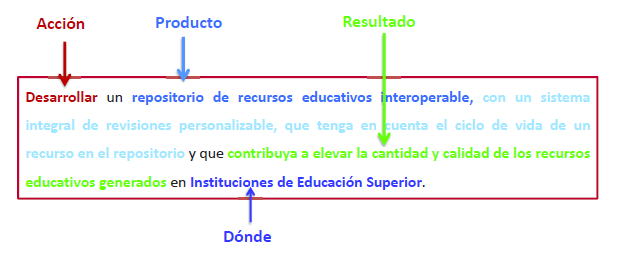
\includegraphics[width=16cm,height=5cm]{Imagenes/Figura12}
			\begin{tablenotes}[para,flushleft]
			{\small
				\textit{\textbf{Nota.}} El gráfico representa la estructura de un objetivo general. La acción responde a qué hacer. El producto a qué se obtiene y refleja de campo de acción que se transforma. El resultado a qué se desea obtener, que debe coincidir con los elementos identificados en el problema y deben ser las variables dependientes si la hipótesis de investigación de del tipo causal. El dónde es específicamente donde se aplica esa solución y que debe estar contemplado en el campo de acción. Tomado de Cañizares, R. (2016), Yanza, A.  (2016).
			}
		\end{tablenotes}
	\end{figure}
	\setlength{\parindent}{1.27cm}Es importante que recuerde la Taxonomía de Bloom: verbos que expresan objetivos en los diferentes niveles del proceso de pensamiento (niveles cognoscitivos), se mencionan los siguientes:
	{\doublespacing
	\begin{itemize}[leftmargin=1.70cm]
		\item[1.]	Conocimiento: Definir, repetir, registrar, memorizar, relatar, subrayar, identificar.
		
		\item[2.]	Comprensión: Interpretar, traducir, describir, reconocer, explicar, expresar, ubicar, informar, revisar.
		
		\item[3.]	Aplicación: Aplicar, emplear, utilizar, dramatizar, ilustrar, operar, dibujar, esbozar.
		
		\item[4.]	Análisis: Analizar, distinguir, diferenciar, inspeccionar, probar, comprar, constatar, criticar, discutir, debatir, examinar.
		
		\item[5.]	Síntesis: Planear, proponer, diseñar, formular, reunir, construir, crear, establecer, organizar, dirigir, preparar.
		
		\item[6.]	Evaluación: Evaluar, juzgar, clasificar, estimar, valorar, calificar, seleccionar, escoger, medir.
		
	\end{itemize}
}
	\setlength{\parindent}{1.27cm}Desde el punto de la Gestión de Proyectos, los objetivos deberán mostrar una estructura SMART, al misma que consiste en: 
{\doublespacing
	\begin{itemize}[leftmargin=1.70cm]
		\item[1.] 	E\textbf{S}PECÍFICO
		
		\item[2.]	\textbf{M}EDIBLE
		
		\item[3.]	\textbf{A}SIGNABLE
		
		\item[4.]	\textbf{R}EALISTA
		
		\item[5.]	BASADO EN EL \textbf{T}IEMPO	
	\end{itemize}
}
	\subsection*{\normalsize \underline{Objetivos específicos}} 
	\addcontentsline{toc}{subsection}{Objetivo específicos} 
	\setlength{\parindent}{1.27cm}Puede haber más de un objetivo específico, estos son los propósitos específicos por las cuales se puede lograr el objetivo general. Los objetivos específicos deben de redactarse de tal manera que puedan ser evaluados y que los mismos sean respondidos en las conclusiones y recomendaciones del trabajo de investigación (Bernal, 2006), también puede utilizar verbos en infinitivo. 
	
	\textbf{Utilizar verbos como:}Situar, identificar, analizar, caracterizar, discriminar, definir, explicar, interpretar, comparar, determinar, relacionar, establecer, conceptualizar, operacionalizar, delimitar; analizar, proponer, presentar. 
	
	\setlength{\parindent}{1.27cm}Como ejemplos de objetivos específicos se mencionan los siguientes:
	
{\doublespacing
	\begin{itemize}[leftmargin=1.70cm]
		\item[1.]	\textbf{Realizar} un diagnóstico del proceso de producción y arquitecturas de los sistemas informáticos existentes.
		\item[2.]	\textbf{Elaborar} el marco teórico de la investigación relacionado con los procesos de producción de las industrias farmacéuticas.
		\item[3.]	\textbf{Diseñar} el modelo computacional de seguimiento y control de la producción de fármacos.
		\item[4.]	\textbf{Implementar} los mecanismos de integración para las distintas aplicaciones que convergen en el proceso de producción.
		\item[5.]	\textbf{Evaluar} la propuesta de solución a través de los métodos científicos definidos en la investigación para determinar su pertinencia y calidad.
	\end{itemize}
}
	\section{\normalsize \centering Alcance del proyecto} 
	\setlength{\parindent}{1.27cm}El alcance describe las fronteras de un proyecto, lo que el proyecto entregará y también lo que no entregará, describe los límites del mismo y lo que el proyecto va a entregar, qué información se necesita y qué partes de la organización se verán afectadas. 
	
	\setlength{\parindent}{1.27cm}El alcance describe el cómo de cada objetivo específico. Los alcances no deben ser sobre dimensionados. Incluya límites y excepciones para el trabajo (restricciones).  Defina los criterios de inclusión, exclusión y aceptación del proyecto. Defina las plataformas de desarrollo y prueba, se recomienda describir los roles y módulos. 
	
		\section{\normalsize \centering Justificación e importancia}
	
	\setlength{\parindent}{1.27cm}Exponga las razones, causas, argumentos que tuvo para realizar esta investigación, desde el punto de vista científico.
	
	\setlength{\parindent}{1.27cm}Plantee la trascendencia y utilidad práctica, teórica o metodológica que proporcionará el trabajo, así como el impacto, relevancia y el aporte que constituirá la investigación.  
	\setlength{\parindent}{1.27cm}A quiénes se van a beneficiar con los resultados. La justificación de la investigación significa \textbf{el ¿por qué?} de la investigación. La justificación de la investigación está en función de varias cuestiones:
{\doublespacing
	\begin{itemize}[leftmargin=1.70cm]
		\item[1.] La conveniencia. ¿¨Para qué sirve la investigación? 
		\item[2.] Relevancia Social ¿Cuál es la trascendencia para la sociedad? 
		\item[3.] Implicaciones Prácticas. ¿Ayudará a resolver algún problema práctico? 
		\item[4.] Valor Teórico. ¿En el campo de la teoría sentará alguna pauta? 
		\item[5.] Utilidad ¿Qué utilidad tendrá la solución de la investigación? 
	\end{itemize}
}	
	
	\section{\normalsize \centering Limitaciones del estudio} 
	Se plantean las posibles dificultades que puedan limitar \setlength{\parindent}{1.27cm}el alcance, el dominio de validez y el cumplimiento de algunos de los objetivos de la investigación, sin afectar su viabilidad (recursos, acceso a la información, tiempo, entre otros). Extensión estimada: Hasta 1 página.
}
\newpage
%%%%%%%%%%%%%%%%%%%%%%%%%%%%%%%%%%%%%%%%%%%%%%%%%%%%%%%%
%%%%%%%%%%%%%%%%%%CAPÍTULO2PAGINA1%%%%%%%%%%%%%%%%%%%%%%
{
	\setlength\headsep{2.95cm}
	\addtolength{\textheight}{-2.45cm}
	\section*{\large \centering CAPÍTULO II \\ MARCO TEÓRICO}
	\addcontentsline{toc}{section}{\normalsize CAPÍTULO II - MARCO TEÓRICO}
	\section{\normalsize \centering Antecedentes del estudio}
	{\setlength{\parindent}{1.27cm}La investigación a realizar debe tener en cuenta el conocimiento previamente construido, pues esta forma parte de una estructura teórica ya existente. El marco teórico implica analizar teorías, investigaciones, antecedentes que se consideren válidos para el encuadre del estudio pues la búsqueda y sistematización de aquellas teorías procedentes pueden ayudar en el análisis del problema a investigar.}
	\section{\normalsize  \centering Fundamentación teórica}
	
	\setlength{\parindent}{1.27cm} Realice una exposición fundamentada en la más amplia bibliografía consultada procurando que esta sea actualizada, sobre el problema que investigará y las variables que maneja.
	
	\setlength{\parindent}{1.27cm}  CCómo se basó en la consulta bibliográfico-documental, aplique las normas de elaboración de referencias y citas basadas en Norma APA7, para que no constituya un plagio o consulte la hoja anexa de este manual.
	
	\setlength{\parindent}{1.27cm} Todo el desarrollo del marco teórico debe responder a las orientaciones filosóficas, psicológicas, sociológicas, pedagógicas, sociales, etc. que usted eligió para fundamentar su investigación.
	
	\setlength{\parindent}{1.27cm} Deberá describir lo más detalladamente posible la situación actual que genera la investigación o el desarrollo de un aplicativo. Debe describir las herramientas y/o técnicas que se emplean para desarrollar la investigación. En caso de temas de desarrollo se deben \hspace{0.1cm} describir
	\newpage
	\restoregeometry
	\justify
	 las plataformas, versiones de software y comparativos para escoger los componentes de la solución. En proyecto de investigación se deberá definir 
	las variables de su investigación que le permitirán generar la hipótesis. En ambos casos, el estudiante debe revisar un número considerable de fuentes primarias y secundarias.  Evitar gráficos que no aporten a la investigación; por ejemplo, logos de productos de software. Se recomienda mínimo 20 páginas para esta sección. \\
	
	 
	\begin{figure}[h]
		\caption{Análisis comparativo: Ionic vs React Native vs Flutter}
		\label{Figura2} %Para referenciar la tabla
		\vspace*{0.1cm}
		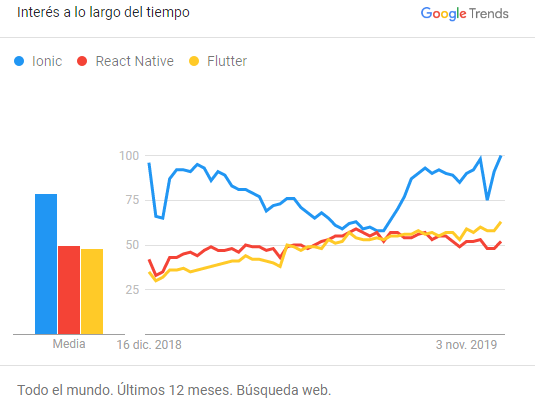
\includegraphics[width=\textwidth]{Imagenes/Figura13}
			\begin{tablenotes}[para,flushleft]
			{\small
				\textit{\textbf{Nota.}} React Native compite con otros frameworks que se encuentran años establecidos en el mercado como lo son Ionic que se encuentra actualmente en su versión 5 y Flutter que le pertenece a Google llevando dos años en el mercado, a pesar de ser un nuevo framework React Native lleva la delantera con respecto al framework de Flutter en tendencia del último año del 2019. Tomado de Morales, L. \& Cruz, J. (2020).
			}
		\end{tablenotes}
	\end{figure}
	
\newpage	

\section{\normalsize  \centering Revisiones sistemáticas}
\vspace*{-0.2cm}

	\setlength{\parindent}{1.27cm}La revisión sistemática forma parte de la investigación secundaria, la cual parte del estudio de las pruebas disponibles sobre una determinada intervención, con el objeto de responder a cuestiones concretas, siguiendo una metodología explícita y rigurosa. La revisión sistemática se ha convertido así en un diseño de investigación en sí misma en el que las unidades de estudio, en lugar de pacientes o unidades administrativas, son los trabajos originales que se revisan.
	
	\setlength{\parindent}{1.27cm}Esquema básico y resumido para la elaboración de una revisión sistemática:
	{\doublespacing
		\begin{itemize}[leftmargin=1.70cm]
			\item[•] Formulación de la pregunta de investigación.
			\item[•] Los criterios de inclusión: metodología del estudio, participantes, intervenciones, comparaciones a estudiar y medidas de resultado. Estas características marcarán el protocolo de estudio y su correcta definición facilitará el resto del proceso.
			\item[•] Búsqueda de estudios en la literatura científica a través de una estrategia de búsqueda que cumpla con los requisitos propuestos, con la lectura del título o el abstract y /o revisando el artículo completo seleccionamos aquellos que reúnen nuestros criterios de selección. Estos estudios constituirán nuestra revisión, de ellos se extraerán los datos necesarios y se evaluarán tanto cualitativa como cuantitativamente.
			\item[•] En los que exista homogeneidad entre los estudios incluidos, y al menos dos de ellos presenten datos razonablemente combinables, se realizará un análisis cuantitativo denominado “metaanálisis”, generalmente mediante la ayuda de programas estadísticos informatizados que facilitan este trabajo, y que permiten visualizar los resultados gráficamente.
			\item[•] Interpretar los resultados obtenidos y extraer las correspondientes conclusiones. 
		
	\end{itemize}
}
		\subsection*{\normalsize \underline{Meta-análisis}}
	\addcontentsline{toc}{subsection}{Meta-análisis}
	
	\setlength{\parindent}{1.27cm} El meta-análisis es un conjunto de herramientas estadísticas, que son útiles para sintetizar los datos de una colección de estudios. El meta-análisis se inicia recopilando estimaciones de un cierto efecto (expresado en un índice de tamaño del efecto, como la diferencia de medias tipificada, la razón de riesgo, o la correlación) de cada estudio. El metaanálisis permite valorar estos efectos en contexto: si el tamaño del efecto es consistente, el efecto del tratamiento puede ser considerado como fuerte y el tamaño del efecto se estima con mayor precisión que con un solo estudio. Si el tamaño del efecto varía, esa variación puede ser descrita y, potencialmente explicada.

\section{\normalsize  \centering Hipótesis / Preguntas científicas a contestarse}	
	
	\setlength{\parindent}{1.27cm} Plantee los supuestos o hipótesis a comprobar o demostrar en la investigación como posibles respuestas al problema. Para hacer el planteamiento correcto acerca de la solución de un problema científico es necesario la formulación de determinadas suposiciones o predicciones, que tiene como punto de partida los conocimientos teóricos y empíricos existentes sobre los hechos y fenómenos que dan origen al problema plateado (Marco Teórico).
	
	\setlength{\parindent}{1.27cm} Solamente plantee las hipótesis si su investigación es de campo. Utilice el título correspondiente: Hipótesis, para investigación de campo, y preguntas científicas si es investigación documental.

	\setlength{\parindent}{1.27cm}  Un ejemplo de pregunta científica a contestarse es: ¿La sistematización de la gestión actual de emisión y validación de certificados para capacitación docente ayudará a mejorar la eficiencia operativa, disminuir gastos y evitar fraudes o inconsistencias en estos documentos?

\section{\normalsize  \centering Variables de la investigación}	
	
	\setlength{\parindent}{1.27cm} Las variables de estudio describen qué se va a medir y cómo se va medir. Deben ser redactadas en forma específica y puntual. Deben describir los conceptos o variables que el investigador tiene en mente, se derivan de los objetivos específicos del trabajo, y debe existir una relación directa entre objetivos y variables.
	
	\setlength{\parindent}{1.27cm} Los requisitos esenciales que toda medición o instrumentos de recolección de datos debe reunir son: confiabilidad y validez. La confiabilidad de un instrumento de medición se refiere al grado en que su aplicación repetida al mismo sujeto u objeto produce resultados iguales. La validez se refiere al grado en que un instrumento realmente mide la variable que pretende medir.
	
\section{\normalsize  \centering Definiciones conceptuales}	
	
	Indique cómo deben ser entendidos e interpretados los términos básicos del estudio, las variables que planteó anteriormente, el sentido en el que serán utilizados y otros términos que emplearon en el proyecto.
	
	\newpage}	
		
%%%%%%%%%%%%%%%%%%%%%%%%%%%%%%%%%%%%%%%%%%%%%%%%%%%%%%%%
%%%%%%%%%%%%%%%%%%CAPÍTULO3_PAGINA1%%%%%%%%%%%%%%%%%%%
{
\setlength\headsep{2.95cm}
\addtolength{\textheight}{-2.45cm}
\section*{\large \centering CAPÍTULO III \\ METODOLOGÍA DE LA INVESTIGACIÓN}
\addcontentsline{toc}{section}{\normalsize CAPÍTULO III - METODOLOGÍA DE LA INVESTIGACIÓN}
		
\setlength{\parindent}{1.27cm}En esta sección incluya uno o dos párrafos de introducción de este capítulo en función de su dominio de conocimiento.
	
		\section{\normalsize \centering Modalidad de la investigación}
\begin{center}
	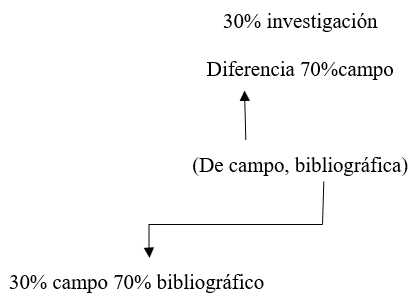
\includegraphics[width=6.5cm,height=4.5cm]{Imagenes/Figura38}
\end{center}

\setlength{\parindent}{1.27cm}En el desarrollo científico e investigativo implica el uso de métodos estadísticos e informáticos que necesitan el acopio de información o datos científicos.  La inferencia estadística no es solo acopio de información científica sino un grupo grande de herramientas analíticas que permiten comprender mejor los sistemas que generan los datos. La información se colecta en forma de muestras o agrupaciones de observaciones de la población y con su estudio se logran resultados confiables, se facilitan los cálculos y la interpretación de los resultados. Explique por qué corresponde a esta modalidad y escriba una cita textual larga de su caracterización.

\section{\normalsize \centering Tipo de investigación}

\setlength{\parindent}{1.27cm}Describa el tipo de investigación que realizará e indique algunas características de ese tipo de investigación. (Exploratorio, descriptivo, explicativo, diagnóstico, evaluativo, de 
\newpage
\restoregeometry
\setlength{\parindent}{0cm}comprobación de hipótesis, causales, experimental, cuasi experimental, correlacionales, ex postfacto, proyectos especiales, proyectos factibles.

\textbf{\underline{Investigación exploratoria}} 
	
\setlength{\parindent}{1.27cm}La investigación exploratoria es un tipo de investigación utilizada para estudiar un problema que no está claramente definido, por lo que se lleva a cabo para comprenderlo mejor, pero sin proporcionar resultados concluyentes, Suele llevarse a cabo cuando el problema se encuentra en una fase preliminar. A menudo, se le llama enfoque de teoría fundamenta: da o investigación interpretativa, ya que se utiliza para responder las preguntas qué, por qué y cómo.

\setlength{\parindent}{1.27cm}Es importante mencionar que la investigación exploratoria se encarga de generar hipótesis que impulsen el desarrollo de un estudio más profundo del cual se extraigan resultados y una conclusión. 

\setlength{\parindent}{0cm}\textbf{\underline{La investigación o método descriptivo de investigación}} 

\setlength{\parindent}{1.27cm}Es el procedimiento usado en ciencia para describir las características del fenómeno, sujeto o población a estudiar. esta no describe por qué ocurre un fenómeno, sino que se limita a observar lo que ocurre sin buscar una explicación.
		
\setlength{\parindent}{0cm}\textbf{\underline{Comprobación de hipótesis}} 
			
\setlength{\parindent}{1.27cm}Una hipótesis de investigación representa un elemento fundamental en el proceso de investigación. Después de formular un problema, el investigador enuncia la hipótesis, que orientará el proceso y permitirá llegar a conclusiones concretas del proyecto que recién comienza. Toda hipótesis constituye un juicio o proposición, una afirmación o una negación de algo. Sin embargo, es un juicio de carácter especial. Las hipótesis son proposiciones provisionales y exploratorias y, por tanto, su valor de veracidad o falsedad depende críticamente de las pruebas empíricas disponibles. En este sentido, la replicabilidad o repetibilidad de los resultados es fundamental para confirmar una hipótesis como solución de un problema.

\setlength{\parindent}{0cm}\textbf{\underline{Investigación evaluativa}} 

		\setlength{\parindent}{1.27cm}La investigación evaluativa es el proceso de evaluar el propósito de una investigación en lugar de un método específico. Consiste en valorar sistemáticamente el mérito del tiempo, el dinero, el esfuerzo y los recursos que utilizados para lograr una meta. Este método mejora el conocimiento y la toma de decisiones, y conduce a aplicaciones prácticas en el mundo real. Además, Se pueden utilizar muchos métodos, como encuestas y experimentos, entre otros.
		
		
\setlength{\parindent}{0cm}\textbf{\underline{Investigación de diagnóstico}} 		

\setlength{\parindent}{1.27cm}La investigación diagnóstica es un método de estudio mediante el cual se logra conocer lo que ocurre en una situación específica. Es decir, se trata del análisis de una serie de sucesos con el objetivo de identificar los factores que promovieron la aparición de un fenómeno. Una de las características principales de la investigación diagnóstica es que analiza cómo se ven afectados los sujetos de estudio por su relación con el entorno y con otros sujetos.
				
\setlength{\parindent}{0cm}\textbf{\underline{Investigación causal}} 				
	
\setlength{\parindent}{1.27cm}La investigación causal es aquella que estudia la relación que se encuentra entre variables. Su objetivo es conocer el efecto positivo o negativo que puede producir un cambio inesperado de las variables independientes. La investigación causal es tanto experimental como estadística, y se puede realizar tanto bajo el control del investigador en un laboratorio o en el campo donde la manipulación se encuentra limitada.
		
		\setlength{\parindent}{1.27cm}Las principales fuentes para obtener información que ayudan al éxito en el proceso de investigación causal son el diseño de preguntas de encuesta que puedan establecer la conexión que existe entre las variables y probar la hipótesis.

\setlength{\parindent}{0cm}\textbf{\underline{Investigación experimental}} 
				
\setlength{\parindent}{1.27cm}La investigación experimental es cualquier investigación realizada con un enfoque científico, donde un conjunto de variables se mantiene constantes, mientras que el otro conjunto de variables se mide como sujeto del experimento. Una verdadera investigación experimental se considera exitosa sólo cuando el investigador confirma que un cambio en la variable dependiente se debe a la manipulación de la variable independiente.

\setlength{\parindent}{0cm}\textbf{\underline{Investigación cuasi experimental}} 
	
\setlength{\parindent}{1.27cm}Su característica más relevante es que no se seleccionan los grupos experimentales de forma aleatoria, sino que se escogen grupos ya formados (por ejemplo, un equipo de fútbol). Se fundamenta en una metodología descriptiva y en algunos elementos cuantitativos y cualitativos, y se utiliza para estudiar diferentes comportamientos, variables sociales.
	
	
\setlength{\parindent}{0cm}\textbf{\underline{Investigación correlacional}} 		
		
\setlength{\parindent}{1.27cm}Es un tipo de método de investigación no experimental en el cual un investigador mide dos variables. Entiende y evalúa la relación estadística entre ellas sin influencia de ninguna variable extraña. La correlación entre dos variables se muestra mediante el coeficiente de correlación (un coeficiente de correlación es una medida estadística que calcula la intensidad de la relación entre dos variables), es decir, un valor medido entre -1 y +1.
		
			\begin{figure}[h]
			\caption{Tipos de investigación}
			\label{Figura3} %Para referenciar la tabla
			\vspace*{0.1cm}
			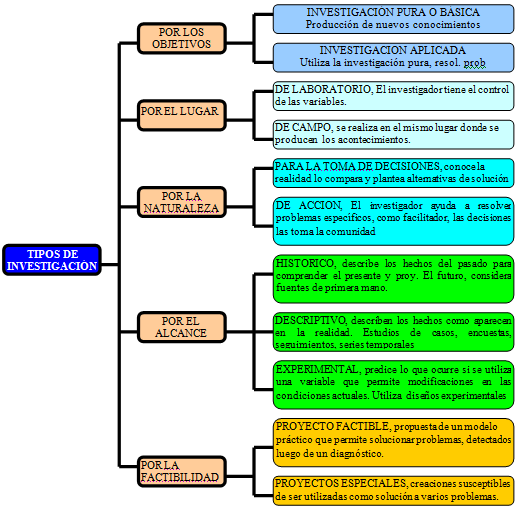
\includegraphics[width=16cm,height=15cm]{Imagenes/Figura37}
			\begin{tablenotes}[para,flushleft]
				{\small
					\textit{\textbf{Nota.}} En esta figura se resumen la tipología de investigaciones, cada una de ellas, con características claramente definidas, que usted deberá evaluar para seleccionarlas y aplicarlas en su proyecto de investigación.
					
				} 
			\end{tablenotes}
		\end{figure}		
		
	\newpage
	
\section{\normalsize \centering Diseño metodológico de la investigación}

		
\setlength{\parindent}{1.27cm}Se enuncia el tipo de diseño y se explican los procedimientos (etapas o secuencia de operaciones) que se seguirán para obtener la información necesaria y procesarla. Cuando sea esto necesario se especificarán, además, los aspectos que constituyen requisitos de las diferentes disciplinas, por ejemplo: Material y Métodos en Ciencias de la Salud y en algunas Ciencias Naturales. Extensión estimada: Hasta 1 página.
		
\subsection*{\normalsize \underline{Metodología de investigación}}
\addcontentsline{toc}{subsection}{Metodología de investigación}	
\setlength{\parindent}{1.27cm}Aplica para proyecto de investigación:
{\doublespacing
\begin{itemize}[leftmargin=1.70cm]
		\item[•] Hipótesis y variables. 
		\item[•] Diseño metodológico.
		\item[•] Tipo de estudio.
		\item[•] Universo y muestra.
\end{itemize}
}
\setlength{\parindent}{1.27cm}La investigación es un proceso sistemático, organizado y objetivo, destinado a responder a una pregunta problema de investigación. La unidad básica del proceso investigativo es el proyecto de investigación, cuyo documento recoge de manera pormenorizada la organización que se ha dado a esta actividad y la forma en que se ejecutará la misma, por lo que representa una guía para el estudiante durante el desarrollo de la investigación.

\setlength{\parindent}{1.27cm}Un proyecto debe contener la siguiente información detallada: título de la investigación, institución responsable de la investigación, resumen, definición y formulación del problema, justificación del estudio, formulación de hipótesis y objetivos, tipo de estudio, universo y muestra, operacionalización de las variables, plan de recolección de datos, plan de procesamiento de la información, consideraciones éticas, recursos, referencias bibliográficas, cronograma, forma de divulgación de los resultados y anexos.

\subsubsection*{\normalsize Población y muestra}
\addcontentsline{toc}{subsubsection}{Población y muestra}	
		
\setlength{\parindent}{1.27cm}\textbf{{\normalsize Población.}} Defina la población en la que realizará la investigación; describa algunas características que le tipifican a la población. (Indique qué profesores o especialistas, consideró en su investigación). Por ejemplo: el caso del criterio de expertos. Si la investigación corresponde a un diseño no experimental (documental o bibliográfico) determine las unidades de análisis utilizadas. Por ejemplo: el uso de un meta-análisis con sus respectivos criterios de inclusión y exclusión. 

\setlength{\parindent}{1.27cm}\textbf{{\normalsize Muestra.}}  Exprese cómo determinó el subconjunto de la población objetivo, a quiénes aplicará los instrumentos para la obtención de la información o datos empíricos, especifique cuál será su población objetivo. Especifique los procedimientos de selección de la muestra si utilizó alguna fórmula y cuáles fueron los resultados. 
		{\doublespacing
			\begin{itemize}[leftmargin=1.70cm]
				\item[•]  Introducción.
				\item[•]  Ponga de título – Población.
				\item[•]  Describa o caracterice a la(s) población(es) que serán utilizadas en la investigación.
				\item[•]  Elabore un cuadro estadístico en el que conste: la población y su número de elementos total; similar al siguiente formato:
				
			\end{itemize}
		}

\begin{table}[h]
	\caption{Definición de la población en el proyecto de investigación}
	\label{Tabla3} %Para referenciar la tabla	
	{\renewcommand{\arraystretch}{1.5} 
		\begin{tabular}{p{10cm}p{5.1cm}}
			\toprule
		\centering	Población&\hspace{0.15cm}N°\\
			\midrule
			\centering.......&....... \\
			\centering.......&....... \\
			\centering.......&....... \\
			 \midrule
			Total&\\
			\midrule
		\end{tabular}
		\begin{tablenotes}[para,flushleft]
			{\small
				\textit{\textbf{Nota.}} En esta tabla se han recopilado datos de fuentes primarias como “nombre de fuente primaria”, la misma que ayudó a identificar la población objetivo del proyecto. La elaboración es propia.
			}
		\end{tablenotes}
	}
\end{table}
	{\doublespacing
\begin{itemize}[leftmargin=1.70cm]
	\item[•]Si las poblaciones son grandes, que pasen de (250) término de referencia, se utilizará la técnica del muestreo.
	\item[•] Ponga de título – Muestra.
	\item[•] Introducción.
	\item[•] Calcule el tamaño de la muestra utilizando cualquiera de las siguientes fórmulas:
\end{itemize}
}
\setlength{\parindent}{1.27cm} Presente el análisis estadístico en cuadros estadísticos (Diagrama de barras, Análisis estadístico descriptivo, prueba de hipótesis). (Indique específicamente quiénes y cuántos 
especialistas o profesores fueron consultados o entrevistados). Para el cálculo del tamaño de la muestra utilice las siguientes fórmulas:

\setlength{\parindent}{1.27cm} 	Para el cálculo de la muestra puede utilizar alguna de las dos fórmulas siguientes: 

\setlength{\parindent}{1.27cm}\textbf{Primer Método}

\setlength{\parindent}{1.27cm}\textbf{UNIVERSIDAD CATÓLICA DE CHILE CIENES}
\vspace*{-0.5cm}
\begin{equation}
n = \frac{PxQxN}{(N-1) E^2 / K^2 + PxQ}
\end{equation}

\begin{flushleft}
	
	\hspace*{4cm}P = Probabilidad de éxito (0.50) \\
	\hspace*{4cm}Q = Probabilidad de fracaso (0.50) \\
	\hspace*{4cm}N = Tamaño de la población (750) \\
	\hspace*{4cm}E = Error de estimación (6\%) \\
	\hspace*{4cm}K = \# de desviac. Típica ``Z" (1:68\%, \textcolor {red}{2:95,5\%}, 3:99.7\%)\\
	\hspace*{4cm}n = Tamaño de la muestra (203)
\end{flushleft}
\vspace*{-0.5cm}
\begin{align*}
n &= \frac{0.50x0.50x750}{(750-1) 0.06^2 / 2^2 + 0.50x0.50}\\
n &= \frac{187.50}{(749)(0.0036) / 4 + 0.25}\\
n &= \frac{187.50}{(749)(0.009) + 0.25}\\
n &= \frac{187.50}{(0.6741) + 0.25}\\
n &= \frac{187.50}{0.9241}\\
n &= 203
\end{align*}
\newpage
\setlength{\parindent}{1.27cm}\textbf{Segundo Método}

\setlength{\parindent}{1.27cm}\textbf{UNIVERSIDAD LIBERTADOR DE VENEZUELA CIRTERPLAN}
\vspace*{-0.8cm}
\begin{equation}
n = \frac{m}{e^2 (m-1) + 1}
\end{equation}

\begin{flushleft}
	\hspace*{4cm}m = Tamaño de la población (750) \\
	\hspace*{4cm}E = error de estimación (6\%) \\
	\hspace*{4cm}n = Tamaño de la muestra (203) 
\end{flushleft}
\vspace*{-0.5cm}	
\begin{align*}
n &= \frac{750}{(0.06)^2 (750 - 1)+1}\\
n &= \frac{750}{(0.0036) (749)+1}\\
n &= \frac{750}{2.6964+1} \\
n &= \frac{750}{3.6964+1} \\
n &= 203
\end{align*}

\setlength{\parindent}{1.27cm}Cálculo de la fracción muestral: 
\vspace*{-0.5cm}
\begin{equation}
f = \frac{n}{N}
\end{equation}
\vspace*{-2cm}
\begin{align*}
f &= \frac{203}{750} = 0.2707
\end{align*}	
\vspace*{-1.5cm}
\begin{table}[h]		
	{\renewcommand{\arraystretch}{0.82} 			
		\caption{Cálculo de la muestra}
		\label{Tabla8} %Para referenciar la tabla
		\begin{center}
			\begin{tabular}{ccc}
				\toprule
				\multicolumn{1}{p{4.50cm}}{\hspace*{1.8cm}Estrato} &\multicolumn{1}{p{3cm}}{\hspace*{0.65cm}Población} &\multicolumn{1}{p{3cm}}{\hspace*{0.7cm}Muestra}  \\
				\midrule
				\multicolumn{1}{c}{Alto} & \multicolumn{1}{c}{120}  &  \multicolumn{1}{c}{32}\\
				
				\multicolumn{1}{c}{Medio} &  \multicolumn{1}{c}{250} & \multicolumn{1}{c}{68} \\
				
				\multicolumn{1}{c}{Bajo} &  \multicolumn{1}{c}{380} & \multicolumn{1}{c}{103}  \\
				
				\multicolumn{1}{c}{\textbf{Total}}&  \multicolumn{1}{c}{\textbf{750}}  & \multicolumn{1}{c}{\textbf{203}}  
				\\ 
				\midrule
			\end{tabular}
		\end{center}	
		\begin{tablenotes}[para,flushleft]
			{\small
				\textit{\textbf{Nota.}} Colocar una descripción de los estratos, población y muestra, según aplique. Es posible mencionar las fuentes de información y criterios que se aplicaron.  						
			}
		\end{tablenotes}
	}
\end{table}		
\clearpage
\subsubsection*{\normalsize Procesamiento y análisis}
\addcontentsline{toc}{subsubsection}{Procesamiento y análisis}	

\setlength{\parindent}{1.27cm}Describa los mecanismos que empleará para el procesamiento de la información sea este manual o mecánico y además los criterios para el análisis de los datos.

\setlength{\parindent}{1.27cm}Análisis por porcentajes, por cuadros (gráficas según objetivos).	

\setlength{\parindent}{1.27cm}\paragraph{Técnicas de recolección de datos}Se describen las técnicas y los instrumentos, que se utilizarán para la obtención de la información, así como los procedimientos de comprobación de  su validez y confiabilidad, según corresponda y si fuese necesario. Los instrumentos empleados se colocarán como anexos. Extensión estimada: Hasta 1 página.

\setlength{\parindent}{2.5cm}\textit{\textbf{Instrumentos de recolección de datos}}
{\doublespacing
\begin{itemize}[leftmargin=2.90cm]
\item[•] \textbf{La técnica ¿qué es?} En conjunto de reglas de sistematización mejoramiento, facilitación y seguridad en el trabajo. Es un conjunto de mecanismos y de máquinas, sistemas y medios de dirigir, recolectar, conservar, reelaborar y transmitir datos, información, energía. Es la estructura del proceso de Investigación.

\begin{center}
	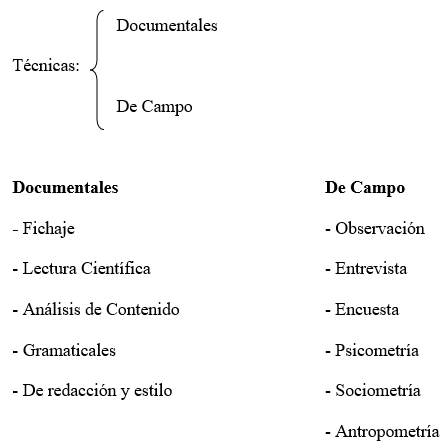
\includegraphics[width=8cm,height=8cm]{Imagenes/Figura39}
\end{center}

\item[•] En el proyecto. Indique con exactitud la (s) técnica (s) de campo que va a utilizar para recolectar la información y datos que requiere para:

\begin{itemize}[leftmargin=0.5cm]
	\item[o] Dar contestación a las preguntas directrices.
	\item[o] Conseguir los objetivos específicos del proyecto.
	\item[o]	Fundamentalmente elaborar el diagnóstico de la necesidad de elaborar la propuesta.
\end{itemize}

\item[•]  \textbf{Los instrumentos ¿qué son? } Herramientas que se utilizan para producir información o datos. Empleados para tener un resultado. Cuando se selecciona una técnica para la recolección de la información que requiere una investigación; ésta, le determina el o los instrumentos que se debe utilizar. Por ejemplo:

\begin{center}
	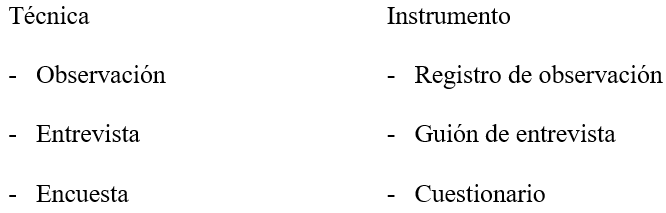
\includegraphics[width=8cm,height=3.5cm]{Imagenes/Figura40}
\end{center}


\end{itemize}
}
\setlength{\parindent}{2.5cm}\textit{\textbf{Instrumentos de la investigación}}
	
\setlength{\parindent}{2.5cm}En esta sección se debe cuestionar lo siguiente:
{\doublespacing
\begin{itemize}[leftmargin=2.90cm]
	\item[•] ¿Qué instrumentos utilizará para obtener la información?
	\item[•] Describa cada instrumento en términos generales.
	\item[•] ¿Cómo construirá y qué criterios utilizará para garantizar la confiabilidad y la validez de los instrumentos?
	\item[•] No se debe anexar los instrumentos porque su elaboración corresponde a la fase ejecutiva.
	
	\setlength{\parindent}{1.80cm}La observación: simple y participante: Entrevistas; cuestionarios; y encuesta. Instrumentos de investigación: Informes instruccionales; Internet. Base de datos científicas Repositorios de tesis.
\end{itemize}
}
\setlength{\parindent}{2.5cm}\textit{\textbf{La encuesta y el cuestionario}}
{\doublespacing
\begin{itemize}[leftmargin=2.90cm]
	\item[•] \textbf{Contenidos.} 
	\begin{itemize}[leftmargin=0.5cm]
		\item[o] Identificación de la Institución.
		\item[o] Objetivo que persigue.
		\item[o] Instrucciones de cómo debe contestar.
		\item[o] Cuestionario o preguntas. – Ítems.
	\end{itemize}
	
	\item[•] \textbf{Utilice:} 
	\begin{itemize}[leftmargin=0.5cm]
		\item[o] Preguntas directas, sencillas y específicas.
		\item[o] Que demanden una sola contestación o respuesta.
		\item[o] Utilice preguntas básicas dentro de su cuestionario (Sexo, Edad).
		\item[o] Utilice preguntas cerradas en el cuestionario (si son de SI y NO, utilice un máximo de 2 preguntas).
		\item[o] Identifique y utilice una variable de respuesta o dependiente, esta deberá ser de tipo dicotómica simple o múltiple).
		\item[o] Elija un mismo tipo de distractores o alternativas. 
		\item[o] El número de preguntas de tipo LIKERT puede formular un mínimo de 7 preguntas y la escala a utilizar por cada pregunta LIKERT debe ser de 1 a 5, siendo 1 la escala más baja y 5 la escala más alta). 
		\item[o] Utilice las preguntas directrices y sus objetivos, para la formulación de las preguntas. 
		\item[o] Elija un formato adecuado, que facilite contestar al investigado y que posteriormente le ayude a procesar la información.
		\item[o] Para el procesamiento de la información utilice programas de software libre como lo es programación en R o Python. 
	
	\end{itemize}

\end{itemize}
}
\setlength{\parindent}{1.27cm}\paragraph{Técnicas estadísticas para el procesamiento de la información}Se describen las técnicas estadísticas que se utilizarán para procesar la información que se obtenga de la aplicación de los instrumentos. Extensión estimada: Hasta 1 página.

\setlength{\parindent}{1.27cm}\textbf{\textit{Técnicas para el Procesamiento y Análisis de Datos. }} Procesar datos significa describir las distintas operaciones a las que serán sometidas los datos recogidos en la investigación.

{\doublespacing
\begin{itemize}[leftmargin=2.90cm]
	\item[•] Proceso a seguir: 
	\begin{itemize}[leftmargin=0.5cm]
		\item[o] Revisión de los instrumentos aplicados.
		\item[o] Tabulación de datos con relación a cada una de las variables previamente identificadas para su análisis estadístico).
		\item[o] Determinación de las frecuencias absolutas, frecuencias relativas.
		\item[o] Diseño y elaboración de cuadros estadísticos con los resultados anteriores, análisis descriptivos de los datos, en caso continúo el cálculo de estadísticos de centralización.
		\item[o]	Elaboración de gráficos: Histograma, Polígono de frecuencias, Ojivas en caso continuo, Gráficos de barras en caso discreto.
	\end{itemize}
	\item Analizar los resultados significa describir, interpretar y discutir los datos numéricos o gráficos que se disponen en los cuadros estadísticos resultantes del procesamiento de datos, para esto debe utilizar paquetes de software libre como lo es R o Python.
	\item El análisis e interpretación debe realizarlo considerando los contenidos del marco teórico y en relación con los objetivos, las variables e indicadores y frecuencias directrices de la investigación.
	\item El producto del análisis constituirá las conclusiones parciales que servirán de insumo para elaborar las conclusiones finales y las recomendaciones.
\end{itemize}
}
\setlength{\parindent}{1.27cm}Se sugiere manejar en una hoja la pregunta, tabla, figura estadística y el análisis respectivo. Como ejemplo se presenta el análisis de la pregunta 4 de una encuesta realizada para recopilar información de un proyecto que consiste en el diseño y desarrollo de un prototipo de aplicación móvil para agilizar el proceso de adopción de mascotas en las distintas fundaciones que existen dentro de la cuidad de Guayaquil. 

\newpage

\setlength{\parindent}{0cm}\textbf{Pregunta 4:} ¿Tiene mascotas en casa actualmente?\\[-0.9cm]

\begin{table}[h]
	{\renewcommand{\arraystretch}{1.2} 		
		\caption{Pregunta 4: ¿Tiene mascotas en casa actualmente?}
		\label{Tabla4} %Para referenciar la tabla	
		
		\begin{tabular}{ccc}
			\toprule
			\multicolumn{1}{p{5cm}}{\hspace*{0.5cm}Opciones de respuesta} &\multicolumn{1}{p{4.75cm}}{\hspace*{0.5cm}Frecuencia Absoluta} & \multicolumn{1}{p{4.90cm}}{\hspace*{0.5cm}Frecuencia Relativa}
			\\
			\midrule
			\multicolumn{1}{c}{Si} & \multicolumn{1}{c}{261}&  \multicolumn{1}{c}{67,80\%}
			\\
			
			\multicolumn{1}{c}{No} &  \multicolumn{1}{c}{124} & \multicolumn{1}{c}{32,20\%}
			
			\\ 
			\midrule
			\multicolumn{1}{c}{Total} & \multicolumn{1}{c}{385} &\multicolumn{1}{c}{100,00\%}
			\\ 
			\midrule
		\end{tabular}
		\begin{tablenotes}[para,flushleft]
			{\small
				\textit{\textbf{Nota.}} En esta tabla se muestran los valores absolutos y relativos correspondientes al proceso de tabulación de la Pregunta 4 aplicada en la encuesta a los 385 individuos seleccionados para la investigación.
			}
		\end{tablenotes}
	}
\end{table}	

\vspace*{-0.1cm}
\begin{figure}[h]
	\caption{Pregunta 4: Análisis gráfico de la pregunta número 4 de la encuesta.}
	\label{Figura5} %Para referenciar la tabla
	\vspace*{0.1cm}
	\begin{center}
		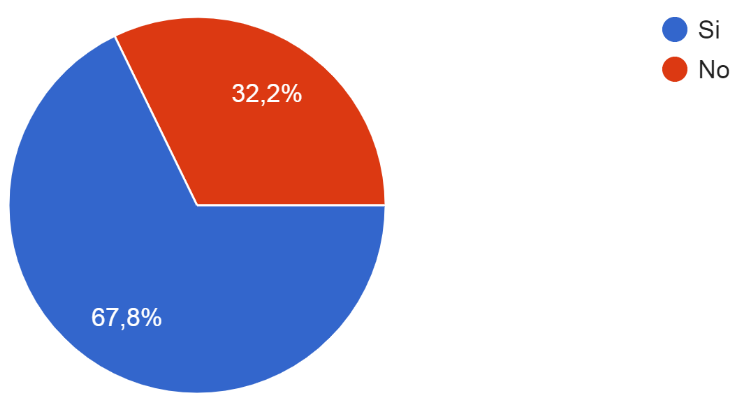
\includegraphics[width=13cm,height=6cm]{Imagenes/Figura31}
	\end{center}
	
	\begin{tablenotes}[para,flushleft]
		{\small
			\textit{\textbf{Nota.}}De un total de 385 encuestados se observa que el 67,80\% indica que dispone de mascotas en casa, mientras que el 32,20\% no las tiene. Se puede mencionar la elaboración de la figura colocando el o los nombres de los investigadores. En el caso de la fuente se puede mencionar el nombre de la institución, base de datos de donde se obtuvo la información, datos propios de la investigación, referencia a otro autor, entre otros. \\
			
		} 
	\end{tablenotes}
\end{figure}	
\vspace*{-1cm}
\setlength{\parindent}{0cm}\textbf{Análisis: }Los resultados de este gráfico muestran un 67,80\% de personas que ya poseen una mascota en casa, las cuales no podrían aplicar a un proceso de adopción al tener ya una mascota en casa. Por ello, las fundaciones utilizan su formulario de adopción para conocer uno de estos aspectos del adoptante que es situación económica al estar estable la fundación de rescate animal permite bajo ese aspecto la adopción, caso contrario los resultados del 32,20\% de personas que no poseen una mascota son totalmente actos bajo este aspecto para realizar el proceso de adopción. 

\newpage

\subsection*{\normalsize \underline{Metodología de gestión del proyecto (opcional)}}
\addcontentsline{toc}{section}{Metodología de gestión del proyecto (opcional)}
\setlength{\parindent}{1.27cm}La Metodología de Marco Lógico (en adelante, MML) es una herramienta para facilitar el proceso de conceptualización, diseño, ejecución y evaluación de proyectos. Su énfasis está centrado en la orientación por objetivos, la orientación hacia grupos beneficiarios y el facilitar la participación y la comunicación entre las partes interesadas. Es un recurso relevante al momento de la formulación de proyectos. Las fases de la MML son:

{\doublespacing
\begin{itemize}[leftmargin=1.70cm]
	
	\item[1.] Definición del problema central.
	\item[2.] Análisis de involucrados.
	\item[3.] Análisis de problemas
	\item[4.] Análisis de objetivos.
	\item[5.] Análisis de Alternativas.
	\item[6.] Diseño de estrategia.
	\item[7.] Matriz de marco lógico.
\end{itemize}
}

\subsubsection*{\normalsize Etapas de la metodología del proyecto }
\addcontentsline{toc}{subsubsection}{Etapas de la metodología del proyecto }

\setlength{\parindent}{1.27cm}Describa las etapas de su proyecto de acuerdo a la metodología de gestión de proyecto utilizada (PMI, CMMI, ITIL, AGILE, entre otras).

\subsection*{\normalsize \underline{Metodología de desarrollo de prototipo (Opcional)}}
\addcontentsline{toc}{section}{Metodología de desarrollo de prototipo (Opcional)}

\setlength{\parindent}{1.27cm}En esta sección deberá argumentar la metodología de desarrollo de software seleccionada, evidenciando la aplicación de la misma dentro del proyecto. Recuerde que cada metodología tiene entregables claros que demostrar. Por ejemplo, para propuestas de desarrollo de software es necesario seguir una metodología de desarrollo (cascada, espiral, prototipado, SCRUM, entre otras). Es importante que se desarrollen las etapas de la metodología considerando aquella que haya sido seleccionada. 

\setlength{\parindent}{1.27cm}Para el \textit{modelo en cascada} se deben identificar claramente las etapas en este capítulo con sus artefactos:
{\doublespacing
\begin{itemize}[leftmargin=1.70cm]
	\item[•] \textbf{Requerimientos: }Documentación formal de requerimientos.
	\item[•]  \textbf{Diseño: }Diagrama de clases, diagrama de arquitectura, diagrama de estados, casos de uso, diagrama de casos de uso.
	\item[•] \textbf{Implementación: } Código. 
	\item[•] \textbf{Verificación: } Casos de Pruebas con resultados de las pruebas.
	\item[•] El cronograma debe mostrar las etapas desarrolladas.
\end{itemize}	
}
\setlength{\parindent}{1.27cm}Para el \textit{modelo prototipo} se deben identificar claramente las etapas en este capítulo con sus artefactos:
{\doublespacing
\begin{itemize}[leftmargin=1.70cm]
	\item[•] \textbf{Requerimientos: }Documentación de requerimientos finales. 
	\item[•] \textbf{Diseño: }Prototipado.
	\item[•] \textbf{Implementación: } Código. 
	\item[•] \textbf{Verificación: } Evaluación de los prototipos.
\end{itemize}
}	
\setlength{\parindent}{1.27cm}En el caso de la \textit{metodología SCRUM (marco de trabajo)}, la cual es frecuentemente utilizada en los proyectos, se deben identificar claramente las etapas en este capítulo con sus artefactos: 
{\doublespacing
\begin{itemize}[leftmargin=1.70cm]
	\item[•] Product Backlog (Historias de usuario completas).
	\item[•] Sprint Backlog.
	\item[•]Incremento/Sprints.
	\item[•] Burndown Chart.
	\item[•] Sprint Planning, gráficas de progreso y demás.
\end{itemize}		
}
\setlength{\parindent}{1.27cm}Ahora bien, comenzar un proyecto tecnológico trae consigo varias interrogantes relacionadas con la Metodología que seguirá. Partiendo de esta premisa, se ha diseñado una metodología para la implementación de proyectos tecnológicos, dividida en fases o etapas y comprende desde el estudio de viabilidad (económica, infraestructura tecnológica), elementos del proyecto (recurso humano, formas de aprendizaje), diseño, evaluación y desarrollo de contenidos, hasta su aplicación.  Recuerde que son aspectos relevantes: Metodología de desarrollo propia del proyecto, supuestos y restricciones, plan de Calidad (Pruebas a realizar).

\setlength{\parindent}{1.27cm}Todos estos elementos se deberán manejar e integrar en el proyecto, bajo criterios de desarrollo y puesta en marcha señalando el orden de intervención y actuación de cada uno. Cabe destacar que para el diseño de la metodología se consideraron los tres ambientes fundamentales que soportan los procesos educativos: laboratorio (investigación y desarrollo), biblioteca (almacenamiento), aula.

		
\section*{\normalsize \centering Beneficiarios directos e indirectos del proyecto}
\addcontentsline{toc}{section}{\textbf{Beneficiarios directos e indirectos del proyecto}}
\setlength{\parindent}{1.27cm}Los beneficiarios, involucrados o stakeholders de un proyecto son las personas u organizaciones que obtendrán algún tipo de beneficio de la implementación del mismo. Se pueden identificar dos tipos de beneficiarios: Directos e indirectos.

\setlength{\parindent}{1.27cm}Beneficiarios directos: Los beneficiarios directos son aquéllos que participarán directamente en el proyecto y, por consiguiente, se beneficiarán de su implementación. Así, las personas que estarán empleadas en el proyecto, que los suplen con materia prima u otros bienes y servicios, o que usarán de alguna manera el producto del proyecto se pueden categorizar como beneficiarios directos. Los pacientes potenciales de una clínica o los niños que posiblemente asistirán a la escuela local (y sus familias) se clasificarían como beneficiarios directos; también, la enfermera o el maestro/maestra que trabajen en la clínica y en la escuela. Los beneficiarios directos de una vía de acceso pueden incluir a las personas que se prevé que la transitarán (conductores y pasajeros), así como a los agricultores y otras personas que empleen camiones para transportar bienes por la carretera.

\setlength{\parindent}{1.27cm}Beneficiarios indirectos: Los beneficiarios indirectos son, con frecuencia, pero no siempre, las personas que viven al interior de la zona de influencia del proyecto. Por consiguiente, aunque una clínica puede prever que tratará únicamente a 1 500 pacientes, los beneficiarios indirectos pueden incluir a las personas que vivan a una distancia de 5, 8 o incluso 10 kilómetros de la clínica (dependiendo de la facilidad de acceso a la misma), pues beneficiará no solamente a los pacientes locales tratados en ese momento sino también a los pacientes potenciales que en un futuro requerirán de tratamiento. Los beneficiarios indirectos de una vía de acceso pueden incluir a todos los habitantes de las comunidades ubicadas en un área cercana a la misma, así como aquéllos que viven a pocos kilómetros a cada lado de la vía.

\setlength{\parindent}{1.27cm}En esta sección se recomienda complementarlo con la Fase 2 de la Metodología de Marco Lógica denominada “Análisis de Involucrados” empleando para ello la identificación, categorización de involucrados, matriz de involucrados, mapa de actores, entre otros.
		
\section*{\normalsize \centering Entregables del proyecto}
\addcontentsline{toc}{section}{Entregables del proyecto}

\setlength{\parindent}{1.27cm}Describa los entregables de su proyecto de acuerdo a la metodología de Proyecto utilizada (PMI, CMMI, ITIL, AGILE, ETC.). Como ejemplo de entregables se menciona: código fuente, código ejecutable, manual técnico, manual de usuario, hardware, manual de instalación y operación, microcontrolador, robot, dispositivo electrónico, acta de entrega/recepción, artículo científico, entre otros.
Actas de entrega/recepción. Para la presentación gráfica y jerárquica de los entregables del proyecto puede hacer uso de la EDT (Estructura de desglose de trabajo).
\newpage
\section{\normalsize \centering Propuesta}
En esta sección deberá describir su propuesta o solución. Es posible que incluya el diseño arquitectónico de su proyecto, modelo construido, prototipo, ajuste esta sección de acuerdo a su producto.

\section*{\normalsize \centering Criterios de validación de la propuesta}
\addcontentsline{toc}{section}{\textbf{Criterios de validación de la propuesta}}
\subsection*{\normalsize \underline{Análisis de datos}}
	
\setlength{\parindent}{1.27cm}	Para proyectos de investigación utilizar Técnicas: En el caso de que se haya hecho una encuesta o se cuente con un Data set, sean estas una combinación de variables cuantitativas y cualitativas. Análisis de la Correlación de Pearson para las variables cuantitativas con su respectivo contraste de hipótesis). Tablas Cruzadas y Análisis de contingencia (Estadístico Chi-cuadrado para el contraste de hipótesis), para variables cualitativas. Para el criterio de la toma de decisiones del estadístico de prueba, debe aplicar contraste de hipótesis.

\setlength{\parindent}{1.27cm}Para este caso se debe tener claro que los resultados obtenidos de la entrevista, será en base al juicio de los expertos, para esto se debe hacer uso de técnicas que me ayuden a validar las respuestas de cada uno de los expertos, para lo cual seguirá los siguientes pasos para validar el cuestionario:
{\doublespacing
\begin{itemize}[leftmargin=1.70cm]
	\item[1.] Selección de los expertos, con un mínimo de 12 a 15 expertos.
	\item[2.] Validación del contenido, en este caso el objetivo es que queden de los 12 expertos una cierta cantidad que cumplan todos los criterios, asegúrese de que después del análisis le queden como mínimo 5 expertos, para esto se utiliza el Método Delphi y la prueba de concordancia de Kendall.
\end{itemize}
}
\setlength{\parindent}{1.27cm}Para el criterio de la toma de decisiones, el estadístico de prueba (Chi-cuadrado), debe aplicar contraste de hipótesis, este es el caso cuando se aplica el Método Delphi y la prueba de concordancia de Kendall.
\setlength{\parindent}{1.27cm}Criterio de toma de decisión en el caso que se utilice el criterio de expertos: 
{\doublespacing
\begin{itemize}[leftmargin=1.70cm]	
	\item[•] Si p $\leq$ 0.05 entonces se rechaza $H_{0}$ y se acepta $H_{1}$ y se dice significativo (Si la probabilidad correspondiente al valor calculado por la prueba estadística es menor o igual que su respectivo valor crítico al nivel de 0.05, entonces se rechaza $H_{0}$ y se dice significativo). 	
	\item[•] Si p $>$ 0.05 entonces se acepta $H_{0}$ y se dice no significativo (Si la probabilidad correspondiente al valor calculado por la prueba estadística es mayor que su respectivo valor crítico al nivel de 0.05, entonces se acepta $H_{0}$ y se dice no significativo).
\end{itemize}	
}
\vspace*{-4mm}
\section*{\normalsize \centering Resultados}
\addcontentsline{toc}{section}{\textbf{Resultados}}
\setlength{\parindent}{1.27cm}Los datos mostrados en la sección resultados deben estar dispuestos de forma clara y sencilla. Los datos mostrados en el texto permiten que el lector capte la información en forma más eficiente y rápida. Las tablas son ideales para presentar datos precisos y repetitivos. Los gráficos son ideales para presentar datos que muestran tendencias o patrones importantes.

\setlength{\parindent}{1.27cm}En esta sección se muestran los hallazgos encontrados en el estudio. Solo se deben mostrar los datos más relevantes. No se interpretan ni comentan los hallazgos. Lo que se coloca dentro del texto, no se debe repetir en las tablas y gráficos. Estos hallazgos deben estar redactados y expresados de manera clara y sencilla, para facilitar la lectura por parte de los lectores ya que es un aporte nuevo para el conocimiento. El autor no necesita incluir los datos obtenidos durante el proceso de investigación, es necesario que escoja lo más significativo, como lo señaló Wesley Powell (1888): “el necio colecciona hechos; el sabio los selecciona”. Si hay variables que no afectan el resultado o influyen de forma negativa, también se deben colocar, no solo es cuestión de colocar los resultados positivos. 

\setlength{\parindent}{1.27cm}Como ejemplo de un resultado se menciona: “33 1/3\% de los ratones utilizados en este experimento curaron con el medicamento ensayado; 33 1/3\% de la población experimental no resultó afectada por el fármaco y persistió en estado agónico; el tercer ratón escapó” (Erwin Neter, Editor Jefe de Infection and Immunity).
\newpage
	\begin{table}[h]
	{\renewcommand{\arraystretch}{0.7}	
		{\singlespacing
	\caption{Términos para definir el rigor científico según el tipo de investigación}
	\label{Tabla4} %Para referenciar la tabla	
		\begin{tabular}{p{4.5cm}cp{4.75cm}}
			\toprule
			\centering Aspecto&Término científico&\hspace{0.5cm}Término naturalístico\\
			\midrule
			\centering Valor verdadero&Validez interna&  \multicolumn{1}{c}{Credibilidad}\\
			\centering Aplicabilidad&Validez externa (generalización)& \multicolumn{1}{c}{Transferencia}\\
			\centering Consistencia&Fiabilidad& \multicolumn{1}{c}{Dependencia}\\
			\centering Neutralidad&Objetividad & \multicolumn{1}{c}{Confirmación}\\
			\midrule
		\end{tabular}
		\begin{tablenotes}[para,flushleft]
			{\small
				\textit{\textbf{Nota.}} Esta tabla plantea los términos para definir el rigor científico según el tipo de investigación que se ha desarrollado. Fuente: Guba / Lincoln (1981/1985, 104).
			}
		\end{tablenotes}
	}
}
\end{table}


}
\newpage
%%%%%%%%%%%%%%%%%%%%%%%%%%%%%%%%%%%%%%%%%%%%%%%%%%%%%%%%
%%%%%%%%%%%%%%%%%%%CÁPITULO4_PAGINA1%%%%%%%%%%%%%%%%%%%%
{

	\setlength\headsep{2.95cm}
	\addtolength{\textheight}{-2.45cm}
	\section*{\large \centering CAPÍTULO IV\\ CONCLUSIONES Y RECOMENDACIONES}
	\addcontentsline{toc}{section}{\normalsize  CAPÍTULO IV - CONCLUSIONES Y RECOMENDACIONES}
	\section{\normalsize \centering Conclusiones}
	\setlength{\parindent}{1.27cm}Una vez realizado el análisis de cada una de las respuestas del instrumento aplicado, se enuncian las conclusiones. Las conclusiones constituyen una sección independiente y presentan, en forma lógica, los resultados del trabajo. Las conclusiones deben ser la respuesta a los objetivos específicos o propósitos planteados. Se debe dar respuesta a todos los objetivos específicos y debe quedar claro de qué manera se evidencia su cumplimiento.  Adicionalmente, pueden agregarse otras conclusiones acerca de los resultados obtenidos.
	
	\setlength{\parindent}{1.27cm}Se recomienda que cada conclusión se maneje en un párrafo independiente, para ello utilice viñetas. Por ejemplo:
	{\doublespacing
		\begin{itemize}	[leftmargin=1.70cm]
			\item[•]Detalle la conclusión 1.
			\item[•]Detalle la conclusión 2.
			\item[•]Entre otras.
		\end{itemize}
	}
	
	\section{\normalsize \centering Recomendaciones}
	
	\setlength{\parindent}{1.27cm}Se presentan como una serie de aspectos que se podría realizar en un futuro en la aplicación, mejora en los procesos administrativos, entre otros. Se incluyen recomendaciones de aspectos que no estuvieron en el alcance pero que se sugieren agregar.
	
	\setlength{\parindent}{1.27cm}Se sugiere que cada recomendación se maneje en un párrafo independiente, para ello utilice viñetas. Por ejemplo:
	
	\newpage
	\restoregeometry
	
	{\doublespacing
		\begin{itemize}	[leftmargin=1.70cm]
			\item[•]	Detalle la recomendación 1.
			\item[•]	Detalle la recomendación 2.
			\item[•]	Entre otras.
		\end{itemize}
	}		
	
	
	\section{\normalsize \centering Trabajos futuros}
	
	\setlength{\parindent}{1.27cm}En esta sección se presentarán las futuras líneas de investigación y/o desarrollo que fueron identificadas durante el período de tiempo que llevó realizar el presente trabajo.
	
	\setlength{\parindent}{1.27cm}Se sugiere que cada idea de trabajo futuro se maneje en un párrafo independiente, para ello utilice viñetas. Por ejemplo:
	{\doublespacing
		\begin{itemize}[leftmargin=1.70cm]
			\item[•]	Detalle el trabajo futuro 1.
			\item[•]	Detalle el trabajo futuro 2.
			\item[•]	Entre otras.
		\end{itemize}
	}	
	
	\newpage

\section*{\large \centering  REFERENCIAS BIBLIOGRÁFICAS}
\addcontentsline{toc}{section}{\normalsize REFERENCIAS BIBLIOGRÁFICAS}

\setlength{\parindent}{1.27cm}Las referencias bibliográficas se asocian a la inclusión de obras o recursos de todos los autores que han sido citados en su trabajo de titulación. Puede incluir artículos de revistas científicas, tesis de grado y/o maestría, libros físicos, libros virtuales, entre otros.

\setlength{\parindent}{1.27cm}Su inclusión es obligatoria en todo trabajo de investigación. Cada referencia bibliográfica se inicia contra el margen izquierdo. Se recomienda el uso de gestores bibliográficos (Mendeley, Zotero, EndNote, entre otros) para su facilidad o gestión.

\setlength{\parindent}{1.27cm}El trabajo de titulación deberá contener al menos 30 referencias bibliográficas correctas. Se recomienda que el 20\% de las referencias sean en idioma inglés.

\setlength{\parindent}{1.27cm}Utilice la norma APA7; por ejemplo, considere las siguientes citas:  Kumar y cols. (2018), Zambrano y Senti (2016). 


\begin{center}
	\textbf{Ejemplo}
\end{center}	

%Se debe habilitar estas líneas de código, para establecer el formato de bibliografía con APA7.
%\bibliographystyle{apacite} 
%\bibliography{BibliografiaProyecto}

\setlength{\parindent}{0cm}Kumar, D., Wu, H., Rajasegarar, S., Leckie, C., Krishnaswamy, S., \& Palaniswami, M. (2018).

\setlength{\parindent}{1.10cm}Fast and scalable big data trajectory clustering for understanding urban mobility. IEEE 

\setlength{\parindent}{1.10cm}Transactions on Intelligent Transportation Systems, 19(11), 3709-3722.

\setlength{\parindent}{0cm}Zambrano, G. R., \& Senti, V. E. (2016). Marco de trabajo para el diseño de una arquitectura  

\setlength{\parindent}{1.10cm}ITS en Ecuador que mejore la interoperabilidad y el despliegue de los sistemas de control 

\setlength{\parindent}{1.10cm}de tráfico vehicular/[Framework for designing an ITS architecture in Ecuador that im- 

\setlength{\parindent}{1.10cm}proves the interoperability and deployment of vehicular traffic control systems]. Interna

\setlength{\parindent}{1.10cm}tional Journal of Innovation and Applied Studies, 14(4), 886.



\newpage
\section*{\large \centering BIBLIOGRAFÍA}
\addcontentsline{toc}{section}{\normalsize BIBLIOGRAFÍA}

La bibliografía es la relación de las fuentes documentales consultadas por el investigador para sustentar sus trabajos. Su inclusión es obligatoria en su trabajo de titulación. Cada referencia bibliográfica se inicia contra el margen izquierdo. Recuerde que solo se refiere a los autores o recursos que se utilizaron, pero que no se citaron en el documento. Puede incluir artículos de revistas científicas, tesis de grado y/o maestría, libros físicos, libros virtuales, entre otros. Utilice la norma APA7.


\begin{center}
	\textbf{Ejemplo}
\end{center}	


\setlength{\parindent}{0cm}Duan, M., Qi, G., Guan, W., \& Guo, R. (2020). Comprehending and Analyzing Multiday Trip-

\setlength{\parindent}{1.10cm}Chaining Patterns of Freight Vehicles Using a Multiscale Method with Prolonged Tra-

\setlength{\parindent}{1.10cm}jectory Data. Journal of Transportation Engineering, Part A: Systems, 146(8), 04020070.

\newpage
\section*{\large\centering ANEXOS}
\addcontentsline{toc}{section}{\normalsize  ANEXOS}
\setlength{\parindent}{1.27cm}Los anexos son todos los contenidos que se agregan al final de un trabajo de titulación para ampliar la información presentada, pero sin resultar imprescindibles para la comprensión del fenómeno estudiado. A continuación, se presenta una lista de los anexos que se sugiere incluir en su proyecto:

\begin{itemize}[leftmargin=1.70cm]
	\item[•]  Anexo 1. Planificación de actividades del proyecto. Se recomienda utilizar Microsoft Project, Gantt Project, TeamGantt, Trello o un software equivalente.
	
	\item[•]  Anexo 2. Geo-localización del problema.
	
	\item[•]  Anexo 3. Carta de autorización del proyecto.
	
	\item[•]  Anexo 4. Fundamentación legal.
	
	\item[•] Anexo 5. Criterios éticos a utilizarse en el desarrollo del proyecto.
	
	\setlength{\parindent}{1.27cm} Se incluye la gestión de permisos a las distintas organizaciones a las cuales se orientan los proyectos para el uso futuro de los datos. Extensión estimada: Hasta 1 página.
	
	
	\item[•] 	Anexo 6. Formato de técnicas de recolección de datos aplicadas para variables cuantitativas o cualitativas.
	
	\item[•] 	Anexo 7. Validación de expertos.
	
	\item[•] 	Anexo 8. Bases de datos para análisis estadístico (Opcional).
	
	\item[•] 	Anexo 9. Diagramas de casos de uso (Dependiendo de la metodología que aplique en el proyecto).
	
	\item[•] 	Anexo 10. Acta de entrega y recepción definitiva.
	
	\item[•] 	Anexo 11. Carta de uso de software (Aplica según se requiera).
	
	\item[•]	Anexo 12. Evidencias fotográficas adicional (Opcional).
	
	\item[•] 	Anexo 13. Manual técnico.
	
	\setlength{\parindent}{1.27cm} El manual incluirá una tabla de contenidos correspondiente.
	
	\item[•] 	Anexo 14. Manual de usuario.
	
	\setlength{\parindent}{1.27cm} El manual incluirá una tabla de contenidos correspondiente.
	
	\item[•] 	Anexo 15. Artículo Científico.
	
	\setlength{\parindent}{1.27cm}El artículo científico requiere revisión y aprobación del docente tutor y revisor del trabajo de titulación. Se deberá seleccionar una revista científica válida para su posterior publicación y adecuar la estructura del artículo en función de la normativa que define dicha revista.
	
	
	
\end{itemize}

\setlength{\parindent}{1.27cm}Considere que si los manuales técnicos y de usuario no superan las 30 páginas pueden ser considerados como anexo, caso contrario deben ser un segundo tomo de su trabajo de titulación. Adicionalmente, recuerde que la cantidad de páginas que suman sus cuatro capítulos no debe ser inferior a 80 páginas.

\newpage
\subsection*{\normalsize \centering Anexo 1. \\ Planificación de actividades del proyecto}
\addcontentsline{toc}{subsection}{Anexo 1. Planificación de actividades del proyecto}
\begin{center}
	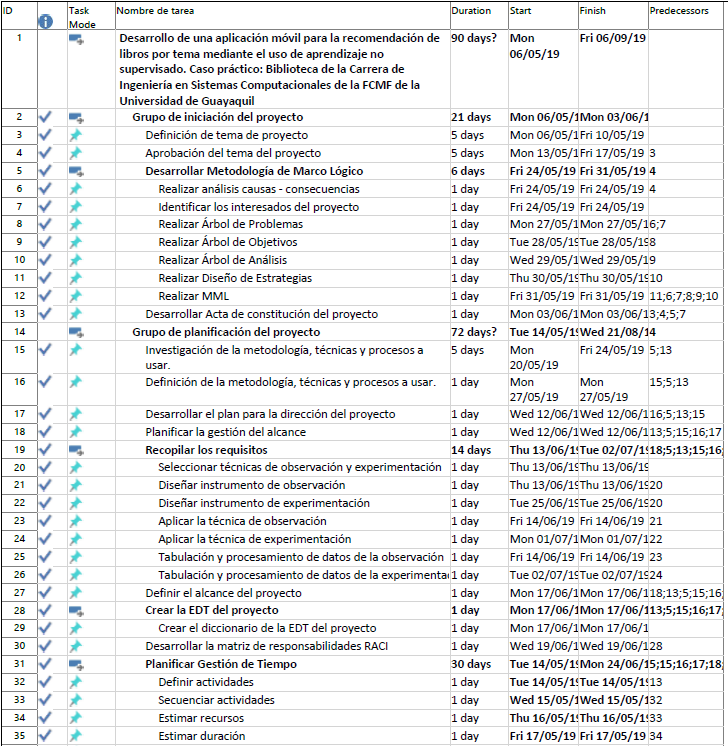
\includegraphics[width=14cm,height=11cm]{Imagenes/Figura32}\\
	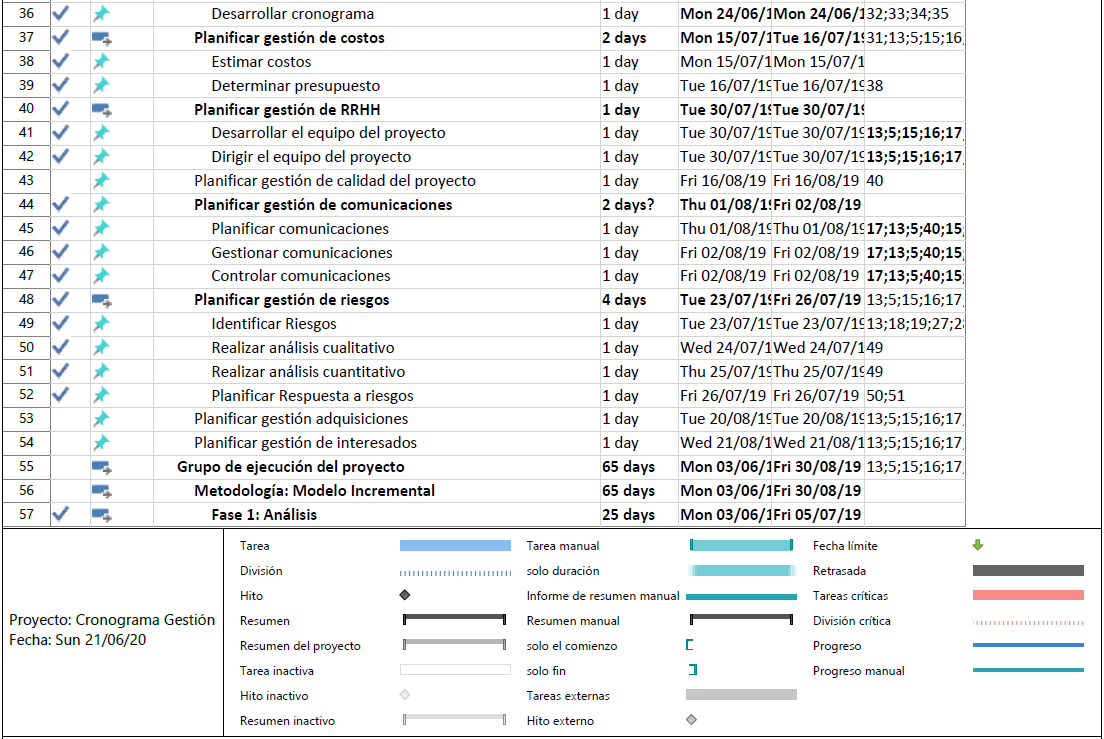
\includegraphics[width=14cm,height=9cm]{Imagenes/Figura33}
\end{center}
\vspace*{-1cm}
\begin{center}
	\singlespacing\textbf{Elaboración:} Investigadores.\\
	\textbf{Fuente:} Propia.
\end{center}
\newpage
\begin{center}
	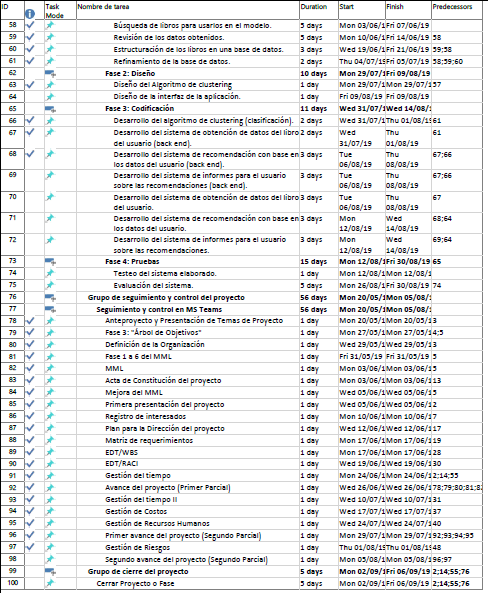
\includegraphics[width=14cm,height=20cm]{Imagenes/Figura34}
\end{center}
\vspace*{-1cm}
\begin{center}
	\singlespacing\textbf{Elaboración:} Investigadores.\\
	\textbf{Fuente:} Propia.
\end{center}
\newpage
\subsection*{\normalsize \centering Anexo 2. \\ Geo-localización del problema}
\addcontentsline{toc}{subsection}{Anexo 2. Geo-localización del problema}
\begin{center}
	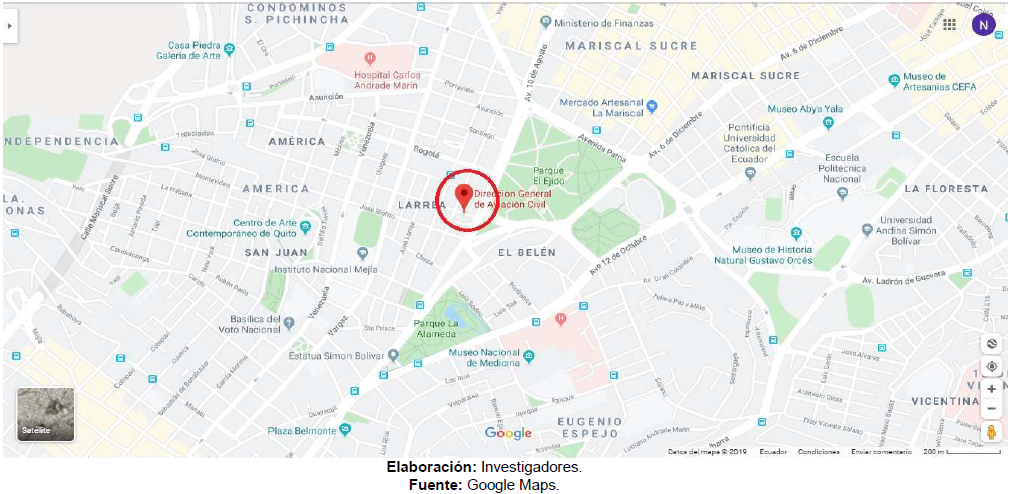
\includegraphics[width=14cm,height=10cm]{Imagenes/Figura35}
\end{center}
\newpage
\subsection*{\normalsize \centering Anexo 3. \\ Carta de autorización del proyecto}
\addcontentsline{toc}{subsection}{Anexo 3. Carta de autorización del proyecto}
\newpage
\subsection*{\normalsize \centering Anexo 4. \\ Fundamentación legal}
\addcontentsline{toc}{subsection}{Anexo 4. Fundamentación legal}
\begin{center}
	Las Normas Legales en un Proyecto de Titulación
\end{center}
Apoyo en leyes, estatutos, acuerdos, reglamentos, especialmente para proyectos especiales y factibles, debe escribir únicamente los artículos citados en la CONSTITUCIÓN DE LA REPUBLICA DEL ECUADOR; LEY ORGÁNICA DE EDUCACIÓN SUPERIOR (art. 21), REGLAMENTO DEL CONSEJO DE EDUCACIÓN SUPERIOR; LEY ÓRGANICA DE TRANSPARENCIA Y ACCESO A LA INFORMACIÓN PUBLICA; LEY DEL SISTEMA NACIONAL DE REGISTRO DE DATOS PÚBLICOS; CÓDIGO ORGÁNICO DE LA ECONOMIA SOCIAL DE LOS CONOCIMIENTOS, CREATIVIDAD E INNOVACIÓN, BUEN VIVIR, etc.\\
$\rightarrow$ Considerar solo artículos relacionados al tema. \\
$\rightarrow$ Debe iniciar la redacción con un breve antecedente de la base legal para realizar el proyecto de titulación. \\
Ejemplo “El presente proyecto de titulación se fundamenta en la constitución, leyes y normas como se detalla a continuación…”.  
\newpage
\begin{table}[h]
	{\renewcommand{\arraystretch}{1.2}	
		{\singlespacing
			\begin{tabular}{|p{4cm}|p{11.1cm}|}
				\hline
				\multicolumn{1}{|p{4cm}|}{ARTÍCULO DE LA LOES} &  \multicolumn{1}{c|}{CONTEXTO} \\
				\hline
				\vspace*{3mm}\centering \footnotesize ¿Qué regula la LOES? ART. 1 ÁMBITO &  Esta Ley regula el sistema de educación superior en el país, a los organismos e instituciones que lo integran; determina derechos, deberes y obligaciones de las personas naturales y jurídicas, y establece las respectivas sanciones por el incumplimiento de las disposiciones contenidas en la Constitución y la presente Ley   ARTICULO 1. \\
				\hline
				\vspace*{-0.5mm}\centering\footnotesize¿Cuál es el Objeto de esta Ley? ART. 2 OBJETO &   \footnotesize Esta Ley tiene como objeto definir sus principios, garantizar el derecho a la educación superior de calidad que propenda a la excelencia, al acceso universal, permanencia, movilidad y egreso sin discriminación alguna.\\
				\hline
				\vspace*{-0.5mm}\centering\footnotesize \underline{Entre las funciones}\newline
				ART. 4 DERECHO A LA EDUCACION SUPERIOR
				&   \footnotesize a) Garantizar el derecho a la educación superior mediante la docencia, la investigación y su vinculación con la sociedad, y asegurar crecientes niveles de calidad, excelencia académica y pertinencia; n) Garantizar la producción de pensamiento y conocimiento articulado con el pensamiento universal; y, ñ) Brindar niveles óptimos de calidad en la formación.\\
				\hline
				\vspace*{12mm}\centering\footnotesize Principio de Igualdad y Principio de Calidad &  \footnotesize El \textbf{principio de igualdad} de oportunidades consiste en garantizar a todos los actores del Sistema de Educación Superior las mismas posibilidades en el acceso, permanencia, movilidad y egreso del sistema, sin discriminación de género, credo, orientación sexual, etnia, cultura, preferencia política, condición socioeconómica o discapacidad.\newline
				El \textbf{principio de calidad} consiste en la búsqueda constante y sistemática de la excelencia, la pertinencia, producción óptima, transmisión del conocimiento y desarrollo del pensamiento mediante la autocrítica, la crítica externa y el mejoramiento permanente
				\\
				\hline
				\vspace*{4mm}\centering\footnotesize ART. 87 &   \footnotesize Como requisito previo a la obtención del título, los y las estudiantes deberán acreditar servicios a la comunidad mediante prácticas o pasantías pre profesionales. debidamente monitoreadas. en los campos de su especialidad, de conformidad con los lineamientos generales definidos por el Consejo de Educación Superior. \\
				\hline
				\footnotesize ARTÍCULO 19.- DEL REGLAMENTO.- NÓMINA DE GRADUADOS Y NOTIFICACIÓN A LA SENESCYT &   \footnotesize Las instituciones de educación superior notificarán obligatoriamente a la SENESCYT la nómina de los graduados y las especificaciones de los títulos que expida, en un plazo no mayor de treinta días contados a partir de la fecha de graduación. (…) este será el único medio oficial a través del cual se verificará el reconocimiento y validez del título en el Ecuador.  \\
				\hline
				\vspace*{5mm}\centering\footnotesize ARTÍCULO 144 PRINCIPIOS
				&   \footnotesize Art. 144.- Tesis Digitalizadas.- Todas las instituciones de educación superior estarán obligadas a entregar las tesis que se elaboren para la obtención de títulos académicos de grado y posgrado en formato digital para ser integradas al Sistema Nacional de Información de la Educación Superior del Ecuador para su difusión pública respetando los derechos de autor.    \\
				\hline
			\end{tabular}
		}
	}
\end{table}

\vspace*{-1cm}
\begin{center}
	\footnotesize
	\singlespacing\textbf{Elaboración:} Investigadores.\\
	\textbf{Fuente:} Ley Orgánica de Educación Superior.
\end{center}

\newpage
\begin{table}[h]
	{\renewcommand{\arraystretch}{1.2}	
		{\singlespacing
			\begin{tabular}{|p{4cm}|p{11.1cm}|}
				\hline
				\multicolumn{1}{|p{4cm}|}{ARTÍCULO DE LA CONSTITUCIÓN} &  \multicolumn{1}{c|}{CONTEXTO} \\
				\hline
				\vspace*{4mm}\centering\footnotesize ARTÍCULO 22 & \footnotesize Establece: las personas tienen derecho a desarrollar su capacidad creativa, al ejercicio digno  y sostenido de las actividades culturales  y artísticas, y a beneficiarse de la protección de los derechos morales y patrimoniales  que les correspondan por las producciones científicas, literarias o artísticas de su autoría. \\
				\hline
				\vspace*{3mm}\centering\footnotesize ARTÍCULO 26 &   \footnotesize La educación es un derecho de las personas a lo largo de su vida y un deber ineludible e inexcusable del Estado. Constituye un área prioritaria de la política pública y de la inversión estatal, garantía de la igualdad e inclusión social y condición indispensable para el buen vivir.\\
				\hline
				\vspace*{2mm}\centering\footnotesize ARTÍCULO 28
				&   \footnotesize La educación responderá al interés público y no estará al servicio de intereses individuales y corporativos. Se garantizará el acceso universal, permanencia, movilidad y egreso sin discriminación alguna\\
				\hline
				\vspace*{8mm}\centering\footnotesize ARTÍCULO 350 &  El sistema de educación superior tiene como finalidad la formación académica y profesional con visión científica y humanista; la investigación científica y tecnológica; la innovación, promoción, desarrollo y difusión de los saberes y las culturas; la construcción de soluciones para los problemas del país, en relación con los objetivos del régimen de desarrollo
				\\
				\hline
				\vspace*{1mm}\centering\footnotesize ARTÍCULO 355 primer y segundo inciso &   \footnotesize El Estado reconocerá a las universidades y escuelas politécnicas autonomía académica, administrativa, financiera y orgánica, acorde con los objetivos del régimen de desarrollo y los principios establecidos en la Constitución \\
				\hline
			\end{tabular}
		}
	}
\end{table}
\vspace*{-1cm}
\begin{center}
	\footnotesize
	\singlespacing\textbf{Elaboración:} Investigadores.\\
	\textbf{Fuente:} Constitución del Ecuador (2010).
\end{center}
\justify
\textbf{FACTIBILIDAD LEGAL.-}\\
Comprende la viabilidad legal del proyecto, es decir, conocer los alcances y limitaciones relacionadas con el desarrollo del mismo.\\
$\rightarrow$ La viabilidad legal busca principalmente determinar la existencia de alguna restricción legal en la realización de un proyecto.\\
$\rightarrow$ Se busca determinar la existencia de normas o regulaciones legales que impidan la ejecución u operación del proyecto.\\
$\rightarrow$ Promover el desarrollo de proyectos sin problemas y dentro de las disposiciones legales.\\
$\rightarrow$ Pueden ser registrados y patentados.\\
$\rightarrow$ Este proyecto no transgrede ninguna norma, leyes o reglamentos establecidos en la Constitución del Ecuador ni en estamentos legales, por tanto, es factible su desarrollo y aplicación.

\textbf{CÓDIGO ORGÁNICO DE LA ECONOMIA SOCIAL DE LOS CONOCIMIENTOS, CREATIVIDAD E INVENCIÓN}\\
\textbf{Artículo 104.- Obras susceptibles de protección.-}La protección reconocida por el presente Título recae sobre todas las obras literarias, artísticas y científicas, que sean originales y que puedan reproducirse o divulgarse por cualquier forma o medio conocido o por conocerse. 12.- SOFTWARE.\\
\textbf{Artículo 131.- Protección de software.-}El software se protege como obra literaria. Dicha protección se otorga independientemente de que hayan sido incorporados en un ordenador y cualquiera sea la forma en que estén expresados, ya sea como código fuente; es decir, en forma legible por el ser humano; o como código objeto; es decir, en forma legible por máquina, ya sea sistemas operativos o sistemas aplicativos, incluyendo diagramas de flujo, planos, manuales de uso, y en general, aquellos elementos que conformen la estructura, secuencia y organización del programa. Se excluye de esta protección las formas estándar de desarrollo de software. En este sentido, los documentos y textos producidos en las Instituciones de Educación Superior desarrollados con el objeto de obtener sus grados académicos y/o trabajos de facultad, son autores intelectuales con el patrocinio de cada institución, por lo tanto, son acreedores a los derechos de protección intelectual dispuestos en la normativa vigente.

\newpage
\subsection*{\normalsize \centering Anexo 5. \\ Criterios éticos a utilizarse en el desarrollo del proyecto}
\addcontentsline{toc}{subsection}{Anexo 5. Criterios éticos a utilizarse en el desarrollo del proyecto}
\vspace*{-1cm}
\begin{table}[h]
	{\renewcommand{\arraystretch}{0.1}	
		{\singlespacing
			\begin{tabular}{|c|c|c|}
				\hline
				\multicolumn{1}{|p{4.50cm}|}{\vspace*{0.2mm}\centering \textbf{Criterios}} & \multicolumn{1}{p{4.50cm}|}{ \centering \textbf{Características del criterio}}& \multicolumn{1}{p{4.50cm}|}{\vspace*{0.2mm}\centering \textbf{Procedimientos}} \\
				\hline
				\multicolumn{1}{|p{4.50cm}|}{\vspace*{3mm}\centering \hspace*{0.5cm}Credibilidad \newline \newline Valor de la verdad/autenticidad} &  \multicolumn{1}{p{4.50cm}|}{\vspace*{0.1mm}Aproximación de los resultados de una investigación frente al fenómeno observado.}& \multicolumn{1}{p{4.50cm}|}{- Los resultados son reconocidos "verdaderos" por los participantes.\newline
					- Observación continua y prolongada del fenómeno. \newline
					- Triangulación.} \\
				
				\hline
				\multicolumn{1}{|p{4.50cm}|}{\vspace*{5mm}\centering \hspace*{0.3cm} Transferibilidad \newline \newline Aplicabilidad} &  \multicolumn{1}{p{5cm}|}{\vspace*{0.1mm}Los resultados derivados de la investigación cualitativa no son generalizables sino transferibles.} & \multicolumn{1}{p{5cm}|}{- Descripción detallada del contexto y de los participantes. \newline - Muestreo teórico. \newline - Recogida exhaustiva de datos.} \\
				
				\hline
				\multicolumn{1}{|p{4.50cm}|}{\vspace*{10mm}\centering \hspace*{0.5cm}Consistencia \newline \newline Dependencia/replicabilidad} &   \multicolumn{1}{p{4.50cm}|}{\vspace*{0.1mm} La complejidad de la investigación cualitativa dificulta la estabilidad de los datos. Tampoco es posible la replicabilidad del estudio.} & \multicolumn{1}{p{4.50cm}|}{- Triangulación  - Empleo de evaluador externo. \newline - Descripción detallada del proceso de recogida, análisis e interpretación de datos. \newline - Reflexibilidad del investigador.} \\
				\hline
				
				\multicolumn{1}{|p{4.50cm}|}{\vspace*{10mm}\centering Confirmabilidad o Reflexibilidad \newline \newline Neutralidad / Objetividad} &  \multicolumn{1}{p{4.50cm}|}{\vspace*{0.1mm} Los resultados de la investigación deben garantizar la veracidad de las descripciones realizadas por los participantes.}& \multicolumn{1}{p{4.50cm}|}{- Transcripciones textuales de las entrevistas.  \newline - Contrastación de los resultados con la literatura existente. \newline - Revisión de hallazgos por otros investigadores. \newline - Identificación y descripción de limitaciones y alcances del investigador.}
				\\
				\hline
				\multicolumn{1}{|p{4.50cm}|}{\vspace*{15mm}\centering Relevancia} &  \multicolumn{1}{p{4.50cm}|}{\vspace*{0.1mm}Permite evaluar el logro de los objetivos planteados y saber si se obtuvo un mejor conocimiento del fenómeno de estudio.}&\multicolumn{1}{p{4.50cm}|}{ - Configuración de nuesvos planteamiento teóricos. o conceptuales. \newline - Comprensión amplia del fenómeno. \newline - Correspondencia entre la justificación y los resultados obtenidos.}
				\\
				\hline
				
				\multicolumn{1}{|p{4.50cm}|}{\vspace*{0.1mm}\centering Adecuación teórica-epistemológica} &  \multicolumn{1}{p{4.50cm}|}{Correspondencia adecuada del problema por investigar y la teoría existente.}& \multicolumn{1}{p{4.50cm}|}{- Contrastación de la pregunta con los métodos. \newline - Ajustes de diseño. }
				\\
				
				\hline
			\end{tabular}
		}
	}
\end{table}
\vspace*{-1cm}
\begin{center}
	\footnotesize
	\singlespacing\textbf{Elaboración:} Investigadores.\\
	\textbf{Fuente:} Propia.
\end{center}



\newpage
\subsection*{\normalsize \centering Anexo 6. \\ Formato de técnicas de recolección de datos aplicadas para variables  cuantitativas o cualitativas \\ }
\addcontentsline{toc}{subsection}{Anexo 6. Formato de técnicas de recolección de datos aplicadas}


\begin{center}
	\textbf{Ejemplo de formato de encuesta}
\end{center}


\includegraphics[width=2cm,height=2cm]{Imagenes/Figura14}
\hspace*{4cm}	
\includegraphics[width=3cm,height=2.5cm]{Imagenes/Figura1}
\hspace*{3.7cm}	
\includegraphics[width=2cm,height=2cm]{Imagenes/Figura15}

{\centering
	\textbf{ UNIVERSIDAD DE GUAYAQUIL} \\[-0.1cm]
	\textbf{ FACULTAD DE CIENCIAS MATEMÁTICAS Y FÍSICAS} \\ [-0.1cm]
	\textbf{ CARRERA DE INGENIERÍA EN SISTEMAS COMPUTACIONALES} \\ [0.5cm]
}
\setlength{\parindent}{0cm}\textbf{Proyecto:} El uso del celular como factor que afecta la comunicación en el entorno familiar.

\setlength{\parindent}{0cm}\textbf{Objetivo:} Recopilar información referente al uso del celular y como afecta la comunicación en el entorno de la familia.\\
De antemano le agradecemos por su valioso tiempo y la formación prestada.\\
La información será tratada de manera confidencial y sólo para propósito investigativo.
\begin{flushright}
	Encuesta N°\rule[0mm]{5mm}{0.1mm}
\end{flushright}	

\textbf{PREGUNTAS BÁSICAS}\\
1.	Edad\rule[0mm]{10mm}{0.1mm}	\\		 
2.	Sexo 	M\rule[0mm]{5mm}{0.1mm}	F\rule[0mm]{5mm}{0.1mm}\\
3.	Lugar de nacimiento \rule[0mm]{10mm}{0.1mm}	\\
4.	Centro educativo en el que se encuentra matriculado su hijo \rule[0mm]{50mm}{0.1mm}	\\
5.	Curso o grado en el que se encuentra matriculado su hijo: \rule[0mm]{10mm}{0.1mm}	Básico\rule[0mm]{10mm}{0.1mm}	 Bachillerato\\
6.	Podría Indicarme, ¿Cuál es el nivel de estudios más alto que ha completado? (Solo marque una respuesta) \\
Universidad \rule[0mm]{5mm}{0.1mm} Tecnología \rule[0mm]{5mm}{0.1mm} Bachillerato \rule[0mm]{5mm}{0.1mm} Primaria Completa\rule[0mm]{5mm}{0.1mm} Primaria sin terminar \rule[0mm]{5mm}{0.1mm} No posee estudios \rule[0mm]{5mm}{0.1mm}

\textbf{PREGUNTAS RESPECTO A LA RELACIÓN FAMILIAR CON SU HIJO} 

7.	Número de miembros de su familia con quien vive (Sin incluirse) \rule[0mm]{5mm}{0.1mm} 

8.	Personas de su familia con quien usted vive (Marque más de una):

Esposo\rule[0mm]{5mm}{0.1mm} Hijo\rule[0mm]{5mm}{0.1mm} Hija\rule[0mm]{5mm}{0.1mm} Padre\rule[0mm]{5mm}{0.1mm} Madre\rule[0mm]{5mm}{0.1mm} Hermanos\rule[0mm]{5mm}{0.1mm}Abuelos\rule[0mm]{5mm}{0.1mm} Otros\rule[0mm]{5mm}{0.1mm}

9.	¿Cómo calificaría la relación que tiene con su hijo? 

Excelente\rule[0mm]{5mm}{0.1mm}	Buena\rule[0mm]{5mm}{0.1mm} Regular\rule[0mm]{5mm}{0.1mm}  Mala\rule[0mm]{5mm}{0.1mm}

10. Continúan más preguntas.


\newpage

\begin{center}
	\textbf{Ejemplo de formato de entrevista}
\end{center}


\includegraphics[width=2cm,height=2cm]{Imagenes/Figura14}
\hspace*{4cm}	
\includegraphics[width=3cm,height=2.5cm]{Imagenes/Figura1}
\hspace*{3.7cm}	
\includegraphics[width=2cm,height=2cm]{Imagenes/Figura15}

{\centering
	\textbf{ UNIVERSIDAD DE GUAYAQUIL} \\[-0.1cm]
	\textbf{ FACULTAD DE CIENCIAS MATEMÁTICAS Y FÍSICAS} \\ [-0.1cm]
	\textbf{ CARRERA DE INGENIERÍA EN SISTEMAS COMPUTACIONALES} \\ [0.5cm]
}
\setlength{\parindent}{0cm}\textbf{Proyecto:} Implementación de un Sistema de Control para el Registro de Capacitaciones en el Área de Meteorología de la Dirección de Aviación Civil.

\setlength{\parindent}{0cm}\textbf{Objetivo:} Realizar un levantamiento de información
sobre los procesos y subprocesos del sistema de capacitación del área de meteorología de la Dirección de Aviación Civil (DAG).\\
De antemano le agradecemos por su valioso tiempo y la formación prestada.\\
La información será tratada de manera confidencial y solo para propósito investigativo.
\begin{flushright}
	Entrevista N°\rule[0mm]{5mm}{0.1mm}
\end{flushright}	

\setlength{\parindent}{0cm}Nombre del entrevistado:	\\
\rule[0mm]{160mm}{0.1mm}	

\setlength{\parindent}{0cm}Área de adscripción \\
\rule[0mm]{160mm}{0.1mm}	

\setlength{\parindent}{0cm}Cargo:\rule[0mm]{100mm}{0.1mm}Fecha:\rule[0mm]{5mm}{0.1mm}/\rule[0mm]{5mm}{0.1mm}/\rule[0mm]{5mm}{0.1mm}Hora:\rule[0mm]{5mm}{0.1mm}:\rule[0mm]{5mm}{0.1mm}

\setlength{\parindent}{1.27cm}1. ¿Todos los cursos son dictados por la Escuela Técnica de Aviación Civil?\\
\rule[0mm]{160mm}{0.1mm}
\rule[0mm]{160mm}{0.1mm}

\setlength{\parindent}{1.27cm}2. ¿En dónde se dan los cursos existe la infraestructura apta para la capacidad del personal que será capacitado? \\
\rule[0mm]{160mm}{0.1mm}
\rule[0mm]{160mm}{0.1mm}

\setlength{\parindent}{1.27cm}3. ¿Son cursos, seminarios o talleres los que realiza la Escuela de Aviación Civil?\\
\rule[0mm]{160mm}{0.1mm}
\rule[0mm]{160mm}{0.1mm}

\setlength{\parindent}{1.27cm}4. Continúan…


\newpage


{\singlespacing \footnotesize
	\begin{turn}{90}
		\renewcommand{\multirowsetup}{\centering}	{\renewcommand{\arraystretch}{1.4}
			\begin{tabular}{|p{5cm}|r|r|r|r|} 
				
				\multicolumn{1}{p{6cm}}{ \vspace*{0.1cm}
\includegraphics[width=6cm,height=1.5cm]{Imagenes/Figura36}} &\multicolumn{3}{p{9.1cm}}{\vspace{0.1mm} Universidad de Guayaquil \newline Facultad de Ciencias Matemáticas y Físicas \newline
					Carrera de Ingeniería en Sistemas Computacionales}
				& 
				\multicolumn{1}{p{4cm}}{\vspace{3mm}
\includegraphics[width=2cm,height=1.5cm]{Imagenes/Figura1}\hspace*{0.5cm}
\includegraphics[width=2cm,height=1.5cm]{Imagenes/Figura14}\hspace*{0.5cm}
\includegraphics[width=2cm,height=1.5cm]{Imagenes/Figura15}}
				\\
				
				\multicolumn{5}{c}{\textbf{Ejemplo de ficha de Observación }}
				\\
				
				\multicolumn{5}{p{24cm}}{\textbf{Proyecto:} Desarrollo de una aplicación móvil para la recomendación de libros por tema mediante el uso de aprendizaje no supervisado. Caso práctico: Biblioteca de la Carrera de Ingeniería en Sistemas Computacionales de la Facultad de Ciencias Matemáticas y Físicas de la Universidad de Guayaquil. }
				\\
				
				\multicolumn{5}{p{24cm}}{\textbf{Objetivo:} Evidenciar el tiempo que se demora cada estudiante al realizar una búsqueda de recursos bibliotecarios. }
				\\
				
				\multicolumn{5}{p{24cm}}{\textbf{Proceso:} Se utilizar esta ficha de observación para contrastar con el proceso de desarrollo de software.}
				\\
				
				\multicolumn{5}{p{24cm}}{\textbf{Lugar:} Biblioteca de la Carrera de Ingeniería en Sistemas Computacionales de la Facultad de Ciencias Matemáticas y Físicas de la Universidad de Guayaquil}
				\\
				
				\multicolumn{4}{p{2cm}}{\textbf{Responsable:}\rule[0mm]{130mm}{0.1mm} } & \multicolumn{1}{l}{\textbf{Fecha:}\rule[0mm]{45mm}{0.1mm}} 
				\\
				\hline
				\multirow{2}{6cm}{Número de Estudiante} & \multicolumn{2}{p{2cm}|}
				{\centering Hora de:
				} & \multirow{2}{1cm}{\hspace*{-5cm}Tarea ejecutada} & \multirow{2}{8cm}{Observaciones}
				
				
				\tabularnewline 
				\cline{2-3}& \multicolumn{1}{p{1cm}|}{\centering \hspace*{-0.35cm} Entrada}  &  \multicolumn{1}{p{1cm}|}{\centering Salida}  & & 
				
				\tabularnewline 
				
				\hline
				
				&&&& \\
				\hline
				&&&&\\
				\hline
				&&&&\\
				\hline
				&&&& \\
				\hline
				&&&& \\
				\hline
				&&&& \\
				\hline
				\multicolumn{5}{c}{}\\
				
				\multicolumn{5}{c}{ \rule[0mm]{45mm}{0.1mm}}\\
				
				\multicolumn{5}{c}{ Firma de responsable} \\
				
				
			\end{tabular}
			
			
		}
		
	\end{turn}
}



\newpage

{\singlespacing \footnotesize
	\begin{turn}{90}
		\renewcommand{\multirowsetup}{\centering}	{\renewcommand{\arraystretch}{1.4}
			\begin{tabular}{|p{5cm}|r|r|r|r|} 
				
				\multicolumn{1}{p{6cm}}{ \vspace*{0.1cm}
\includegraphics[width=6cm,height=1.5cm]{Imagenes/Figura36}} &\multicolumn{3}{p{9.1cm}}{\vspace{0.1mm} Universidad de Guayaquil \newline Facultad de Ciencias Matemáticas y Físicas \newline
					Carrera de Ingeniería en Sistemas Computacionales}
				& 
				\multicolumn{1}{p{4cm}}{\vspace{3mm}
\includegraphics[width=2cm,height=1.5cm]{Imagenes/Figura1}\hspace*{0.5cm}
\includegraphics[width=2cm,height=1.5cm]{Imagenes/Figura14}\hspace*{0.5cm}
\includegraphics[width=2cm,height=1.5cm]{Imagenes/Figura15}}
				\\
				
				\multicolumn{5}{c}{\textbf{Ejemplo de ficha de Experimentación }}
				\\
				
				\multicolumn{5}{p{24cm}}{\textbf{Proyecto:} Desarrollo de una aplicación móvil para la recomendación de libros por tema mediante el uso de aprendizaje no supervisado. Caso práctico: Biblioteca de la Carrera de Ingeniería en Sistemas Computacionales de la Facultad de Ciencias Matemáticas y Físicas de la Universidad de Guayaquil. }
				\\
				
				\multicolumn{5}{p{24cm}}{\textbf{Lugar:} Biblioteca de la Carrera de Ingeniería en Sistemas Computacionales de la Facultad de Ciencias Matemáticas y Físicas de la Universidad de Guayaquil}
				\\
				
				\multicolumn{5}{p{24cm}}{\textbf{Proceso de Experimentación:} Preguntarle a un estudiante al entrar en la biblioteca si va a hacer una investigación con los libros de la universidad, en caso de respuesta positiva se le pide que instale la aplicación móvil para que esta le ayude a agilizar el proceso, luego de esto, se recolectan datos de cuanto tiempo pasa dentro de la biblioteca para luego contrastar estos datos con los tiempos de investigación de los estudiantes antes del desarrollo de la aplicación esto sirve para enfocarnos en el proceso de entrenamiento. }
				\\
				
				\multicolumn{4}{p{2cm}}{\textbf{Responsable:}\rule[0mm]{130mm}{0.1mm} } & \multicolumn{1}{l}{\textbf{Fecha:}\rule[0mm]{45mm}{0.1mm}} 
				\\
				\hline
				\multirow{2}{6cm}{Número de Estudiante} & \multicolumn{2}{p{2cm}|}
				{\centering Hora de:
				} &\multicolumn{2}{p{10cm}|}{ \hspace*{6.5cm}Observaciones} 
				
				
				
				\tabularnewline 
				\cline{2-3}& \multicolumn{1}{p{1cm}|}{\centering \hspace*{-0.35cm} Entrada}  &  \multicolumn{1}{p{1cm}|}{\centering Salida}  &\multicolumn{2}{p{2cm}|}{}  
				
				\tabularnewline 
				
				\hline
				
				&&&\multicolumn{2}{c|}{}\\
				\hline
				&&&\multicolumn{2}{c|}{}\\
				\hline
				&&&\multicolumn{2}{c|}{}\\
				\hline
				&&&\multicolumn{2}{c|}{} \\
				\hline
				&&&\multicolumn{2}{c|}{} \\
				\hline
				\multicolumn{5}{c}{} \\
				
				
				\multicolumn{5}{c}{ \rule[0mm]{45mm}{0.1mm}}\\
				
				\multicolumn{5}{c}{ Firma de responsable} \\
				
				
			\end{tabular}
			
			
		}
		
	\end{turn}
}


\newpage
\subsection*{\normalsize \centering Anexo 7. \\ Validación de expertos} 
\addcontentsline{toc}{subsection}{Anexo 7. Validación de expertos}
\justify
\textbf{Juicios de Expertos}\\
Para la validación del proyecto se utilizó el instrumento de juicio de expertos con la finalidad de realizar las pruebas de funcionalidad y porcentaje de validación del software desarrollado, adicional los expertos que realicen la validación correspondiente pueda ofrecer valorización para este proyecto y que las técnicas implementadas sean las adecuadas. (Véase Anexo 7).\\
Considere de 3 a 5 validación de expertos.

\newpage
\begin{turn}{90}
	
	
	\renewcommand{\multirowsetup}{\centering}	{\renewcommand{\arraystretch}{0.42}
		\begin{tabular}{|p{3.3cm}|l|r|r|r|r|r|r|r|r|r|r|r|r|r|r|r|r|r|r|r|r|}
			\multicolumn{22}{c}{\textbf{ANEXO 7. VALIDACIÓN DE EXPERTOS}}\\
			\multicolumn{22}{l}{\textbf{DATOS GENERALES}}\\
			\hline
			\multicolumn{4}{|p{6cm}|}{\textbf{APELLIDOS Y NOMBRES DEL EXPERTO}} & \multicolumn{8}{p{6cm}|}{\textbf{TITULO PROFESIONAL DEL EXPERTO}} & \multicolumn{10}{c|}{\textbf{AUTOR(ES)}}\\
			\hline
			\multicolumn{4}{|l|}{} & \multicolumn{8}{l|}{} & \multicolumn{5}{l|}{}& \multicolumn{5}{l|}{} \\
			\hline
			\multicolumn{4}{|c|}{\textbf{TÍTULO DEL PROYECTO}} &  \multicolumn{18}{l|}{}\\
			\hline
			\multirow{3}{2.5cm}{\textbf{INDICADOR}} & \multirow{3}{2.5cm}{\textbf{CRITERIO}} & \multicolumn{4}{p{3cm}|}
			{\centering \textbf{DEFICIENTE 0-20}
			}
			& \multicolumn{4}{p{3cm}|}
			{\centering \textbf{REGULAR 21-40}
			}
			& \multicolumn{4}{p{3cm}|}
			{\centering \textbf{BUENA	\\ 41-60}
			}
			& \multicolumn{4}{p{3cm}|}
			{\centering \textbf{MUY BUENA61-80}
			}
			& \multicolumn{4}{p{3cm}|}
			{\centering \textbf{EXCELENTE 81-100}
			}
			\tabularnewline 
			\cline{3-22}&  & \multicolumn{1}{p{0.4cm}|}{\centering 5} & \multicolumn{1}{p{0.4cm}|}{\centering 10}& \multicolumn{1}{p{0.4cm}|}{\centering 15}& \multicolumn{1}{p{0.4cm}|}{\centering 20}& \multicolumn{1}{p{0.4cm}|}{\centering 25}& \multicolumn{1}{p{0.4cm}|}{\centering 30}& \multicolumn{1}{p{0.4cm}|}{\centering 35}& \multicolumn{1}{p{0.4cm}|}{\centering 40}& \multicolumn{1}{p{0.4cm}|}{\centering 45}& \multicolumn{1}{p{0.4cm}|}{\centering 50}& \multicolumn{1}{p{0.4cm}|}{\centering 55}& \multicolumn{1}{p{0.4cm}|}{\centering 60}& \multicolumn{1}{p{0.4cm}|}{\centering 65}& \multicolumn{1}{p{0.4cm}|}{\centering 70}& \multicolumn{1}{p{0.4cm}|}{\centering 75}& \multicolumn{1}{p{0.4cm}|}{\centering 80}& \multicolumn{1}{p{0.4cm}|}{\centering 85}& \multicolumn{1}{p{0.4cm}|}{\centering 90}& \multicolumn{1}{p{0.4cm}|}{\centering 95}& \multicolumn{1}{p{0.4cm}|}{\centering 100}	
			\tabularnewline 
			\hline
			\footnotesize CLARIDAD &\multirow{-4.5}{3cm}{\singlespacing \justify \scriptsize Se utiliza el lenguaje de programación apropiado que facilita la comprensión.}&&&&&&&&&&&&&&&&&&&&\\
			&&&&&&&&&&&&&&&&&&&&&\\
			&&&&&&&&&&&&&&&&&&&&&\\
			\hline
			\footnotesize OBJETIVIDAD&\multirow{-4.4}{3cm}{\singlespacing \justify \scriptsize Está expresado en conductas observables y medibles}.&&&&&&&&&&&&&&&&&&&&\\
			&&&&&&&&&&&&&&&&&&&&&\\
			&&&&&&&&&&&&&&&&&&&&&\\
			\hline
			\footnotesize ACTUALIDAD&\multirow{-4.5}{3cm}{\singlespacing \justify \scriptsize Esta acorde a los aportes recientes en la disciplina de  estudio.}&&&&&&&&&&&&&&&&&&&&\\
			&&&&&&&&&&&&&&&&&&&&&\\
			&&&&&&&&&&&&&&&&&&&&&\\
			\hline
			\footnotesize SUFICIENCIA&\multirow{-4.5}{3cm}{\singlespacing \justify \scriptsize Son suficientes la cantidad  y calidad de ítems  presentados en el  instrumento.}&&&&&&&&&&&&&&&&&&&&\\
			&&&&&&&&&&&&&&&&&&&&&\\
			&&&&&&&&&&&&&&&&&&&&&\\
			\hline
			\footnotesize INTENCIONALIDAD&\multirow{-4.5}{3cm}{\singlespacing \justify \scriptsize Es adecuado para valorar la variable seleccionada.}&&&&&&&&&&&&&&&&&&&&\\
			&&&&&&&&&&&&&&&&&&&&&\\
			&&&&&&&&&&&&&&&&&&&&&\\
			\hline
			\footnotesize CONSISTENCIA&\multirow{-4.5}{3cm}{\singlespacing \justify \scriptsize Está basado en aspectos teóricos y científicos.}&&&&&&&&&&&&&&&&&&&&\\
			&&&&&&&&&&&&&&&&&&&&&\\
			&&&&&&&&&&&&&&&&&&&&&\\
			\hline
			\footnotesize METODOLOGÍA &\multirow{-4.5}{3cm}{\singlespacing \justify \scriptsize El instrumento se relaciona con el método planteado en el proyecto}&&&&&&&&&&&&&&&&&&&&\\
			&&&&&&&&&&&&&&&&&&&&&\\
			&&&&&&&&&&&&&&&&&&&&&\\
			\hline
			\footnotesize APLICABILIDAD&\multirow{-4.5}{3cm}{\singlespacing \justify \scriptsize El instrumento es de fácil aplicación.}
			&&&&&&&&&&&&&&&&&&&&\\
			&&&&&&&&&&&&&&&&&&&&&\\
			\hline
			
		\end{tabular}
	}
\end{turn}



\newpage
\begin{center}
	\textbf{CONSTANCIA DE JUICIO DE EXPERTO}
\end{center}
\vspace*{0.5cm}
\setlength{\parindent}{0cm}Estimado(a) Ingeniero(a)\\
Nombres y apellidos del tutor(a)\\
DOCENTE TUTOR(A) DEL TRABAJO DE TITULACIÓN\\
Ciudad.-
\vspace*{0.5cm}

\setlength{\parindent}{1.27cm}El presente instrumento certifica que se realizó la revisión del proyecto de titulación “NOMBRE DEL PROYECTO” cuyos criterios e indicadores empleados permitieron articular el trabajo según se muestra en el Anexo 7, por tanto, \rule[0mm]{60mm}{0.1mm} y 
\rule[0mm]{60mm}{0.1mm} estudiante(s) no titulados de la Carrera de Ingeniería en Sistemas computacionales de la Universidad de Guayaquil, (\textbf{NO}) pueden continuar con el proceso de titulación en vista que (no) existen observaciones.\\
\rule[0mm]{160mm}{0.1mm}\\
\rule[0mm]{160mm}{0.1mm}\\
\rule[0mm]{160mm}{0.1mm}\\
\rule[0mm]{160mm}{0.1mm}

\setlength{\parindent}{1.27cm}Por lo actuado en el Anexo 7, se procede a validar el trabajo de titulación. 

\setlength{\parindent}{0cm}Sin otro particular.
\vspace*{1cm}

\begin{center}
	\singlespacing
	\rule[0mm]{70mm}{0.1mm}\\
	\textbf{Nombres y apellidos del experto}  \\
	\textbf{C.I. N°}9999999999   
\end{center}

\vspace*{1cm}
\begin{center}
	\footnotesize
	\singlespacing\textbf{Elaboración:} Investigadores.\\
	\textbf{Fuente:} Propia.
\end{center}


\newpage
\begin{center}
	\textbf{INSTRUMENTO DE VALIDACIÓN}
\end{center}
\vspace*{-0.5cm}
{\singlespacing
	\setlength{\parindent}{0cm}  Estimado(a) participante:
	
	\setlength{\parindent}{0cm} Usted ha sido seleccionado(a)  para ser parte de la prueba piloto del instrumento que se adjunta a continuación, por lo que le solicito muy comedidamente responder el cuestionario, anotar el tiempo en que tardo en contestarlo, para luego llenar el cuadro propuesto.
	
	\begin{table}[h]
		{\renewcommand{\arraystretch}{1}	
			{\singlespacing
				\begin{tabular}{|p{1cm}|p{1.25cm}|c|p{1.25cm}|c|p{1.75cm}|c|c|}
					\hline
					\multicolumn{8}{|c|}{INSTRUMENTO DE VALIDACIÓN}  \\
					\hline
					\multicolumn{8}{|l|}{TÍTULO DEL TRABAJO: ""}  \\
					\hline
					\multicolumn{8}{|l|}{INSTRUCTIVO}  \\
					\hline
					& \multicolumn{2}{p{3cm}|}{\centering Congruencia  (con el título del trabajo)}  &\multicolumn{2}{p{3cm}|}{\centering  Claridad}&\multicolumn{2}{p{4cm}|}{Tendenciasidad (las preguntas estan libres de otros factores que influyen en la respuesta)}& \multicolumn{1}{p{2.71cm}|}{Observaciones} \\
					\hhline{|-|-|-|-|-|-|-|}
					\footnotesize Item &   \footnotesize Si & \footnotesize \hspace*{-0.9cm}No & \footnotesize Si & \footnotesize  \hspace*{-0.9cm} No &\footnotesize Si&\footnotesize \hspace*{-0.9cm} No&\\
					\hline
					\footnotesize 1 &   \footnotesize  &&&&&& \\
					\hline
					\footnotesize 2 &  \footnotesize  &&&&&& \\
					\hline
					\footnotesize 3 &   \footnotesize  &&&&&&\\
					\hline
					\footnotesize 4 &   \footnotesize  &&&&&&\\
					\hline
					\footnotesize 5 &   \footnotesize  &&&&&&\\
					\hline
					\footnotesize 6 &   \footnotesize  &&&&&&\\
					\hline
					\footnotesize 7 &   \footnotesize  &&&&&&\\
					\hline
					\footnotesize 8 &   \footnotesize  &&&&&&\\
					\hline
					\footnotesize 9 &   \footnotesize  &&&&&&\\
					\hline
					\footnotesize 10 &   \footnotesize  &&&&&&\\
					\hline
					\footnotesize 12 &   \footnotesize  &&&&&&\\
					\hline
					\footnotesize 13 &   \footnotesize  &&&&&&\\
					\hline
					\footnotesize 14 &   \footnotesize  &&&&&&\\
					\hline
					\footnotesize 15 &   \footnotesize  &&&&&&\\
					\hline
					\footnotesize Total &   \footnotesize  &&&&&&\\
					\hhline{|-|-|-|-|-|-|-|}
					\footnotesize \% &   \footnotesize &&&&&& \\
					\hline
					\multicolumn{8}{l}{} \\		
					
				\end{tabular}
				
				\begin{tabular}{|p{2.5cm}|r|r|r|r|r|r|r|} 
					
					\hline
					\multirow{4}{2cm}{\textbf{EVALUADO POR}} & \multicolumn{3}{p{5.15cm}|}
					{\centering \textbf{}
					}
					& \multicolumn{2}{p{4cm}|}
					{\centering \textbf{}
					}
					& \multicolumn{2}{p{2.5cm}|}
					{\centering \textbf{}
					}
					\tabularnewline 
					\cline{2-7}& \multicolumn{3}{p{5.15cm}|}{\centering Apellido(s) Nombre(s)} & 
					\multicolumn{2}{p{4cm}|}{\centering Cédula de Identidad} 
					& \multicolumn{1}{p{2.5cm}|}
					{\centering Fecha Firma
					}
					\tabularnewline 
					\cline{2-7}& \multicolumn{3}{p{5.15cm}|}{\centering } & 
					\multicolumn{2}{p{4cm}|}{\centering } 
					& \multicolumn{1}{p{2.5cm}|}
					{\centering 
					}
					\tabularnewline
					\cline{2-7}& \multicolumn{3}{p{5.15cm}|}{\centering Profesión} & 
					\multicolumn{2}{p{4cm}|}{\centering Cargo} 
					& \multicolumn{1}{p{2.5cm}|}
					{\centering Teléfono
					}
					\tabularnewline
					\hline
				\end{tabular}	
			}
		}
	\end{table}
}
\vspace*{-0.4cm}
Agradecido por su colaboración

Cordialmente,

\vspace*{-0.4cm}
\begin{center}
	\singlespacing
	\rule[0mm]{70mm}{0.1mm}\\
	\textbf{Nombres y apellidos}  \\
	\textbf{C.I. N°}9999999999   
\end{center}
\vspace*{-0.5cm}
\begin{center}
	\footnotesize
	\singlespacing\textbf{Elaboración:} Investigadores.\\
	\textbf{Fuente:} Propia.
\end{center}



\newpage
\subsection*{\normalsize \centering Anexo 8. \\ Bases de datos para análisis estadístico (Opcional)}
\addcontentsline{toc}{subsection}{Anexo 8. Bases de datos para análisis estadístico (Opcional)}	
\vspace*{0.2cm}
\begin{center}
	\textbf{BASE DE DATOS DE LAS VARIABLES DE ESTUDIO}   \\
	\vspace*{1cm}
	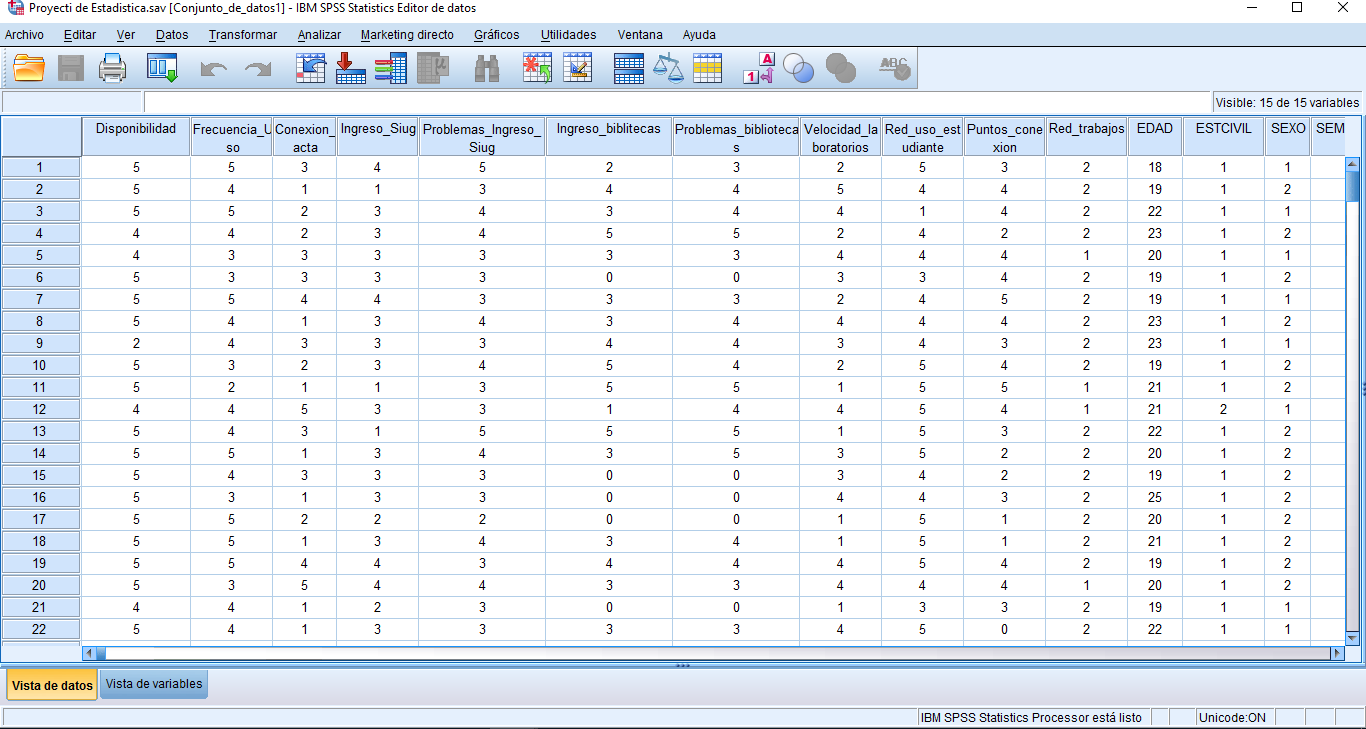
\includegraphics[width=14cm,height=8cm]{Imagenes/Figura16} \\
	\vspace*{1cm}
	\textbf{CODIFICACIÓN DE LAS VARIABLES EN SPSS} \\
	\vspace*{1cm}
	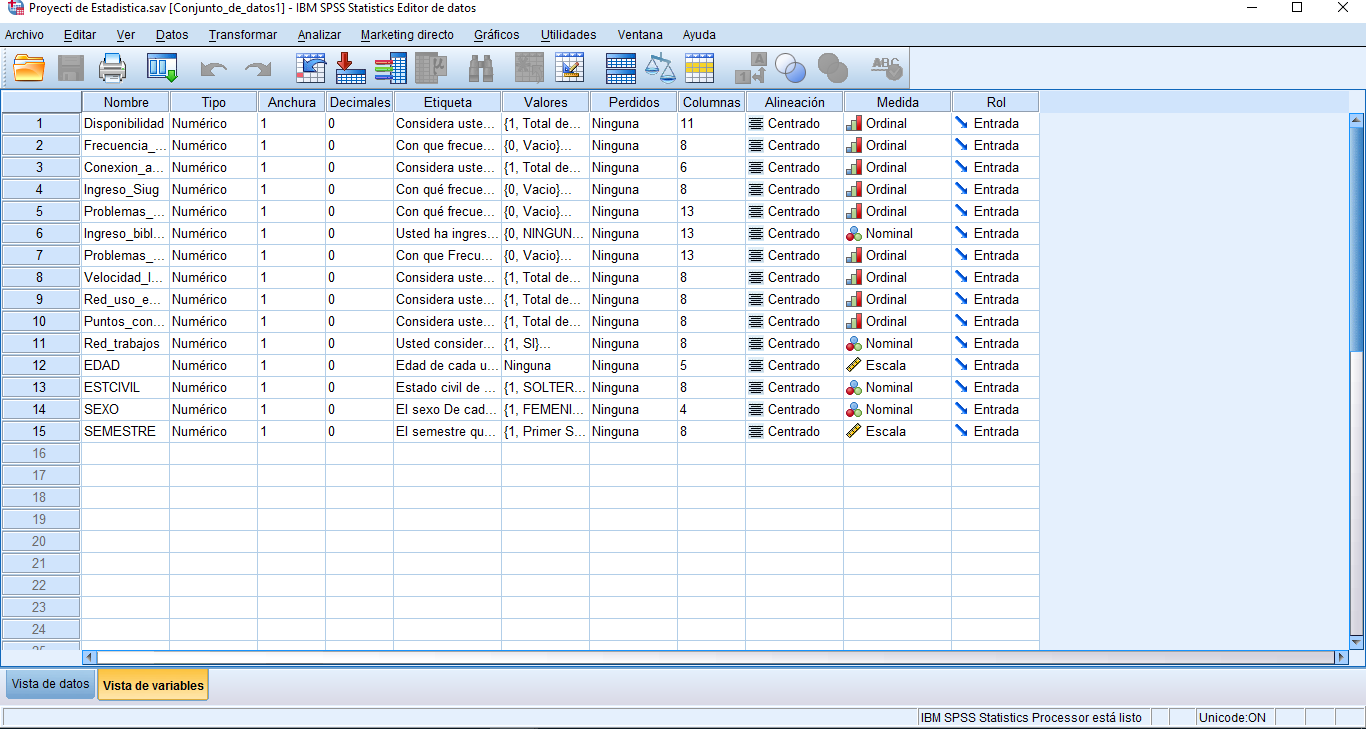
\includegraphics[width=14cm,height=8cm]{Imagenes/Figura17}
	
\end{center}
\newpage
\textbf{Definición de Variables} (Un concepto básico de lo que hace cada variable)\\
\textbf{Variables Cuantitativas}
\begin{itemize}
	\item[•] \textbf{Edad:} Esta variable discreta nos indica la edad de los estudiantes encuestados.
	\item[•] \textbf{Semestre:} Indica si la mayor cantidad de estudiantes encuestados
	
\end{itemize}
\textbf{Variables Cualitativas}
\begin{itemize}
	\item[•]\textbf{Sexo:} Indica si el estudiante encuestado es del sexo masculino o femenino.
	\item[•] \textbf{Estado civil:} Indica si el estudiante encuestado es: casado, soltero o unión libre.
	\item[•] \textbf{Dispositivo\_Conexion\_WIFI:} Nos indica si están de acuerdo en un dispositivo capacitado (Hotspot) para conectarse a la red WIFI.
	\item[•] \textbf{Frecuencia\_Uso:} Indica la frecuencia que le da un estudiante promedio a la red para uso de investigaciones respecto a la carrera.
	\item[•] \textbf{Red\_Apta:} Indica la opinión del estudiante encuestado si se encuentra totalmente de acuerdo o en desacuerdo sobre si la conectividad es la suficiente para realizar sus trabajos.
	\item[•] \textbf{Frecuencia\_Problemas\_SIUG:} Indica que tan frecuente ha sido las molestias al tratar de ingresar al sitio web del SIUG.
	\item[•] \textbf{Ingreso\_Bibliotecas:} Indica si el estudiante ha ingresado al menos una vez a una biblioteca de la carrera.
	\item[•] \textbf{Problemas\_Bibliotecas:} Indica si al ingresar a las bibliotecas ha tenido siempre o nunca problemas en la conexión.
	\item[•] \textbf{Velocidad\_Laboratorios:} Indica la opinión del estudiante encuestado sobre si la velocidad de navegación en los Laboratorios de la carrera son óptimos para la realización de trabajos.
	\item[•] \textbf{Uso\_Exclusivo:} Indica la opinión del estudiante si se encuentra de acuerdo o no en que se implemente más puntos de conexión en la CINT solo para estudiantes y otro solo para docentes para que de esta manera mejore la velocidad de navegación y con ella la efectividad de la misma.
	\item[•] \textbf{Puntos\_conexion\_Suficientes:} Indica la opinión del estudiante si está conforme o no con la cantidad de puntos de acceso a la red WIFI en la CINT.
	\item[•] \textbf{Red\_Optima:} Indica la opinión si el estudiante sobre que si la red es óptima para su uso académico.
	\item[•] \textbf{Conocimiento\_Previo:} Indica si el estudiante tenía conocimiento de las bibliotecas virtuales de la CINT antes de esta encuesta.
\end{itemize}
\newpage
\justify
\textbf{Variables Cualitativas}
\textbf{Tabla de codificación la variable SEXO}
\begin{center}
	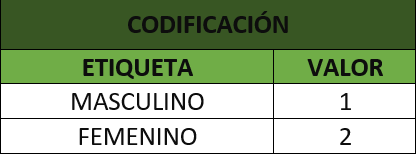
\includegraphics[width=6cm,height=2cm]{Imagenes/Figura18}
\end{center}
\textbf{Tabla de codificación la variable ESTADO CIVIL}
\begin{center}
	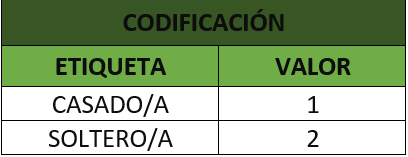
\includegraphics[width=6cm,height=2cm]{Imagenes/Figura19}
\end{center}
\textbf{Tabla de codificación la variable DISPOSITIVO\_CONEXION\_WIFI}
\begin{center}
	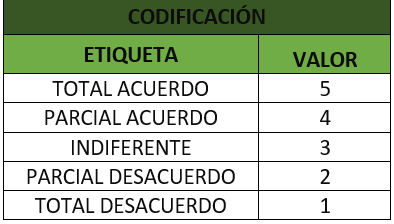
\includegraphics[width=7cm,height=4cm]{Imagenes/Figura20}
\end{center}
\textbf{Tabla de codificación la variable FRECUENCIA\_USO}
\begin{center}
	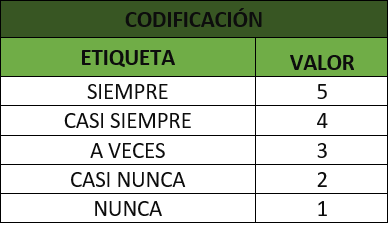
\includegraphics[width=7cm,height=4cm]{Imagenes/Figura21}
\end{center}
\textbf{Tabla de codificación la variable FRECUENCIA\_PROBLEMAS\_SIUG}
\begin{center}
	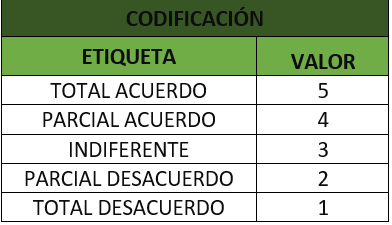
\includegraphics[width=7cm,height=4cm]{Imagenes/Figura22}
\end{center}
\newpage
\textbf{Tabla de codificación la variable INGRESO\_BIBLIOTECAS}
\begin{center}
	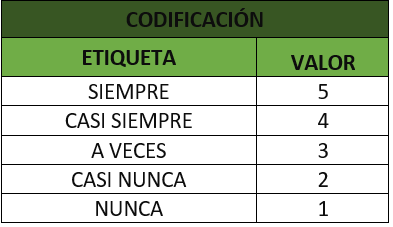
\includegraphics[width=7cm,height=4cm]{Imagenes/Figura23}
\end{center}
\textbf{Tabla de codificación la variable PROBLEMAS\_BIBLIOTECAS}
\begin{center}
	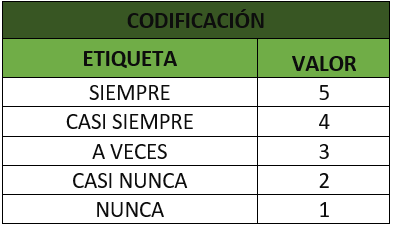
\includegraphics[width=7cm,height=4cm]{Imagenes/Figura24}
\end{center}
\textbf{Tabla de codificación la variable VELOCIDAD\_LABORATORIOS }
\begin{center}
	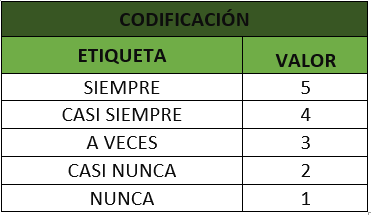
\includegraphics[width=7cm,height=4cm]{Imagenes/Figura25}
\end{center}
\textbf{Tabla de codificación la variable USO\_EXCLUSIVO}
\begin{center}
	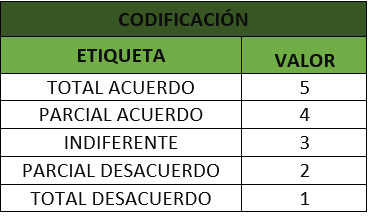
\includegraphics[width=7cm,height=4cm]{Imagenes/Figura26}
\end{center}
\newpage
\textbf{Tabla de codificación la variable PUNTOS\_CONEXION\_SUFICIENTES}
\begin{center}
	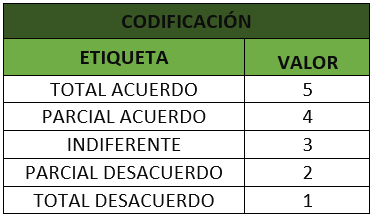
\includegraphics[width=7cm,height=4cm]{Imagenes/Figura27}
\end{center}

\textbf{Tabla de codificación la variable RED\_OPTIMA}

\begin{center}
	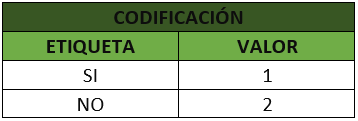
\includegraphics[width=6cm,height=2cm]{Imagenes/Figura28}
\end{center}

\textbf{Tabla de codificación la variable CONOCIMIENTO\_PREVIO}
\begin{center}
	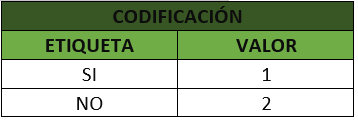
\includegraphics[width=6cm,height=2cm]{Imagenes/Figura29}
\end{center}

\clearpage


\begin{center}
	\textbf{EJEMPLO DE FORMATO DE TABLA DE META-ANÁLISIS} 
\end{center}

\begin{center}
	{\scriptsize \singlespacing
		
		\renewcommand{\multirowsetup}{\centering}	{\renewcommand{\arraystretch}{1.5}
			\begin{tabular}{|p{2.5cm}|p{4cm}|p{1cm}|p{0.5cm}|p{1.5cm}|p{3.5cm}|}
				
				\hline
				\vspace*{5mm}\centering \textbf{Autores} & 	\vspace*{5mm}\centering \textbf{Resumen} & 	\vspace*{2mm}\centering \textbf{Tipo de Publicación} & 	\vspace*{5mm}\centering \textbf{Año} & \centering \textbf{Se Aplicó Análisis Digital de Imágenes (DIC)} & 	{\vspace*{2.5mm}\centering 
					\textbf{Características importantes ADI}} \\
				\hline
				"F. Laurin, 
				J.-S. Charrier, D. Lévêque, J.-F. Maire, A. Mavel, P. Nuñez"
				&Presentan en su investigación el daño provocado después de un impacto en los diseños de estructuras de materiales compuestos laminados con fibra de carbono y matriz polimérica en la elaboración de aviones civiles.
				&Artículo
				&2012
				&Si
				&Análisis de imágenes también permite estimar la evolución de la densidad de fisuras en las estructuras de material compuesto.
				\\
				\hline
				J. Wang, A. M. Waas, y H. Wang
				&En su trabajo presentan los resultados de un estudio experimental y numérico del comportamiento de impacto de baja velocidad de paneles sándwich de material compuesto laminado, con centro de espuma. Los paneles con núcleo de espuma de poliuretano y tejido de laminado de carbono. 
				&Artículo
				&2013
				&Si
				&Análisis de imágenes también permite estimar la evolución de la densidad de fisuras en las estructuras de material compuesto.
				\\
				\hline	
			\end{tabular}
			
		}
		
	}
\end{center}			

\begin{center}
	
	{\scriptsize \singlespacing
		\renewcommand{\multirowsetup}{\centering}	{\renewcommand{\arraystretch}{1.5}
			\begin{tabular}{|p{2cm}|p{2cm}|p{2.5cm}|p{2cm}|p{2cm}|p{2.5cm}|}
				\hline
				\vspace*{0.5mm}\centering  \textbf{Aplicaciones prácticas del Trabajo de Investigación} & \vspace*{0.5mm}\centering  \textbf{Componente específico aplicado para el análisis} & \vspace*{0.5mm}\centering  \textbf{Mecanismos de Daño producido por el impacto} & \vspace*{0.5mm}\centering  \textbf{Tipo de Validación de otra técnica Experimental Utilizada} & \vspace*{0.5mm}\centering \textbf{Evaluación de la otra ténica Experimental Utilizada} &
				{\vspace*{0.5mm}\centering \textbf{Condiciones de contorno del imapacto (campos extraidos)}}	\\
				\hline
				
				Aviones
				& La fabricación de estructuras primarias tales como la caja central del ala y el fuselaje de las alas. 
				& Carga de tracción en la fibra, comprensión después del impacto.
				&1,- Sensor LVDT (linear variable differential transformer) 2,- Medidores de deformación.
				&Medir el desplazamiento de la estructura y medir la rigidez local del material.
				&Desplazamiento y deformación.
				\\
				\hline
				Paneles sándwich
				&Aplicaciones Aeronáuticas.
				&Hendiduras permanentes que tienen formas semiesféricas en el marco del impactador, el aplastamiento de la matriz debido a la compresión, roturas de remolque, fractura de la fibra y la deformación residual global de todo el panel. 
				&Microscopía óptica y electrónica de barrido.
				& Evaluar el área de daño y los patrones de fallas alrededor de la zona afectada, dentro del panel tamaño del impactador, la energía del impacto, El grosor de la cara-hoja, y el grosor del núcleo.
				&Sometidas a impacto de baja velocidad con impactadores de acero hemisférico de diferentes diámetros en los distintos niveles de energía.
				\\
				\hline
				
			\end{tabular}
		}
	}
\end{center}	

\vspace*{-1cm}
\begin{center}
	\singlespacing\textbf{Elaboración:} Investigadores.\\
	\textbf{Fuente:} Propia.
\end{center}

\newpage
\subsection*{\normalsize \centering Anexo 9. \\ Diagramas de casos de uso (Dependiendo de la metodología que aplique en el proyecto)}
\addcontentsline{toc}{subsection}{Anexo 9. Diagramas de casos de uso (Dependiendo de la metodología que aplique en el proyecto)}
\newpage
\subsection*{\normalsize \centering Anexo 10. \\ Acta de entrega y recepción definitiva }
\addcontentsline{toc}{subsection}{Anexo 10. Acta de entrega y recepción definitiva}
\vspace*{0.5cm}

\setlength{\parindent}{1.27cm}La legislación vigente en materia de propiedad intelectual no reconoce ni niega la existencia de una obligación cierta de entrega de los códigos fuente de páginas web. En cambio, en materia contractual civil y mercantil sí se reconoce esta obligación en determinados casos, a saber:
{\doublespacing	
	\begin{itemize}[leftmargin=1.70cm]	
		\item[•]Cuando se haya acordado expresamente la entrega de los códigos fuente.
		\item[•]Cuando no se haya acordado, únicamente en los casos que reúnan las condiciones siguientes:
		\begin{itemize}
			\item[•]La página web debe haber sido personalizada a petición del cliente y para cumplir los fines requeridos por éste.
			\item[•]El comprador queda dependiente del programador para la realización de todo tipo de actualizaciones.
			\item[•]El cliente debe haber corrido con los gastos de investigación y desarrollo de la página web
		\end{itemize}
	\end{itemize}
}
\setlength{\parindent}{0cm}Fuente:\\ {\footnotesize\url{https://www.pablofb.com/2008/11/debo-dar-al-cliente-el-codigo-fuente/}}

\newpage

\begin{flushright}
	En la ciudad de Guayaquil, a \rule[0mm]{10mm}{0.1mm} días del mes de \rule[0mm]{10mm}{0.1mm} de 20 \rule[0mm]{10mm}{0.1mm}
\end{flushright}
Por el presente documento. \\

\setlength{\parindent}{1.27cm}Los estudiantes no titulados de la Carrera de Ingeniería en Sistemas Computacionales \rule[0mm]{60mm}{0.1mm} con cédula de identidad N° \rule[0mm]{50mm}{0.1mm} y \rule[0mm]{60mm}{0.1mm} con cédula de identidad N° \rule[0mm]{50mm}{0.1mm} hacemos la entrega del código fuente del proyecto de titulación a la Dirección de la Carrera de Ingeniería en Sistemas Computacionales en un medio magnético.

\setlength{\parindent}{1.27cm}Los códigos del Programa/producto que se encargaron por compromiso al estar inserto en el proceso de titulación desde fecha \rule[0mm]{10mm}{0.1mm} de \rule[0mm]{20mm}{0.1mm}.

\setlength{\parindent}{1.27cm}Para efectos de dar cumplimiento a la entrega del código fuente, cedo todos los derechos de explotación sobre el programa y, en concreto, los de transformación, comunicación pública, distribución y reproducción, de forma exclusiva, con un ámbito territorial nacional.

\begin{center}
	\vspace*{1cm}
	\singlespacing\rule[0mm]{68mm}{0.1mm} \hspace*{1.8cm} \rule[0mm]{58mm}{0.1mm}\\
	\hspace*{-0.1cm}Nombres y apellidos del estudiante
	\hspace*{3.4cm} Cédula de identidad N°
	
	\vspace*{1cm}
	{\color{red}\rule[0mm]{68mm}{0.1mm}} \hspace*{1.8cm} {\color{red}\rule[0mm]{58mm}{0.1mm}}\\
	\hspace*{-0.1cm}{\color{red}Nombres y apellidos del estudiante}
	\hspace*{3.4cm}{\color{red}Cédula de identidad N°}
\end{center}

\vspace*{2cm}
\begin{center}
	\singlespacing\textbf{Elaboración:} Investigadores.\\
	\textbf{Fuente:} Propia.
\end{center}


\newpage
\subsection*{\normalsize \centering Anexo 11. \\ Carta de uso de software (Aplica según se requiera)}
\addcontentsline{toc}{subsection}{Anexo 11. Carta de uso de software (Aplica según se requiera)}


\begin{flushright}
	Guayaquil, \rule[0mm]{10mm}{0.1mm} de \rule[0mm]{10mm}{0.1mm} de 20 \rule[0mm]{10mm}{0.1mm}
\end{flushright}

\setlength{\parindent}{0cm}Señores\\
\textbf{UNIVERSIDAD DE GUAYAQUIL} \\
Ciudad.- \\

\setlength{\parindent}{1.27cm}Como es de vuestro conocimiento, los estudiantes no titulados \rule[0mm]{60mm}{0.1mm} y  \rule[0mm]{60mm}{0.1mm}, luego de haber realizado su proyecto de titulación cuyo tema es “\rule[0mm]{80mm}{0.1mm}” en nuestra institución \rule[0mm]{60mm}{0.1mm} y dado que para estos fines, se proporcionó información de nuestra base de datos y procesos, además de otros requerimientos que demandaron los estudiantes, creemos pertinente solicitar a ustedes, como Institución de Educación Superior Universidad de Guayaquil, se nos permita hacer uso de una licencia del módulo o sistema desarrollado por los estudiantes, en retribución al trabajo realizado y tiempo invertido de ambas partes, dejando en claro que las puertas de la empresa \rule[0mm]{60mm}{0.1mm}  están abiertas para impulsar nuevos desafíos, con miras de hacer innovación tecnológica con sus estudiantes.

\setlength{\parindent}{1.27cm}Sin otro particular, y en espera de una respuesta favorable quedamos de ustedes muy agradecidos.

\setlength{\parindent}{0cm}Atentamente,
\begin{center}
	\singlespacing
	\rule[0mm]{80mm}{0.1mm} \\
	\textbf{Gerente General o Representante Legal}\\
	\textbf{Empresa XYZ}\\
	\textbf{C.I.N°} 9999999999
\end{center}



\newpage
\subsection*{\normalsize \centering Anexo 12. \\ Evidencias fotográficas adicionales (Opcional)}
\addcontentsline{toc}{subsection}{Anexo 12. Evidencias fotográficas adicionales (Opcional)}

\setlength{\parindent}{0cm}Las imágenes utilizadas en cualquier trabajo al igual que cualquier otra información, debe ser citada adecuadamente siguiendo al manual de Estilo APA.

\begin{itemize}[leftmargin=0.5cm]
	\item[•] Evalúe si es necesario la presencia de esa Imagen o foto en su trabajo.
	\item[•] La imagen debe de ser citada dentro del texto y debe contar con su entrada en las referencias.
	\item[•] Toda fotografía de menores de edad en cualquier contexto, con cualquier tipo de plano que se publique en cualquier medio digital debe tener una autorización firmada por los padres o tutores.
	\item[•] En caso de que se quiera publicar constantemente fotos de los mismos niños, puedes firmar un acuerdo abierto con los padres que especifique dónde se van a publicar, durante qué periodo de tiempo y en qué circunstancias concretas. También podrías agregar algunas prohibiciones para especificar que no pondrás en riesgo su identidad. Piensa por ejemplo en la página de Facebook de un centro de cuidado infantil que constantemente sea alimentado con fotos de los alumnos. Si debes pedir autorización por cada foto seguro tardarás mucho, pero si puedes pedir a los padres que firmen una carta, a inicio de año cuando inscriban a sus hijos, en los que aceptan que publicarás fotos únicamente en la página y que solo estarán relacionadas a las actividades que realizan en el centro.
	\item[•] Hay que tener mucho cuidado con el tipo de imágenes que se publican porque se trata de una población vulnerable que puede ser afectada en sus derechos. 
	\item[•] En las leyes de Ecuador se hace referencia a la prohibición de usar imágenes de menores de edad cuando estos sean víctimas de algún delito.
\end{itemize}
El Código de la Niñez y Adolescencia y un artículo similar se puede observar en la Ley Orgánica de Comunicación.
\begin{itemize}[leftmargin=0.5cm]	
	\item[•] Por último, si obligatoriamente necesitas publicar una imagen de la que tienes duda que puede afectar o no a un niño siempre podrás hacer uso del desenfoque o “blureado” para ocultar su rostro.
\end{itemize}
Ejemplo
\vspace*{0.2cm}

\begin{figure}[h]
	\caption{Descripción breve pero completa que explique la imagen o fotografía.}
	\label{Figura5} %Para referenciar la tabla
	\vspace*{0.1cm}
	\begin{center}
		\centering 
\includegraphics[width=4cm,height=4cm]{Imagenes/Figura41}
	\end{center}
	
	\begin{tablenotes}[para,flushleft]
		{\small
			\textit{\textbf{Nota.}} Incluir una descripción de la imagen que presenta. Se puede enfatizar el objetivo que persigue, la fuente de donde extrajo la fotografía, la elaboración de la misma citada en formato APA7.
		}
	\end{tablenotes}
\end{figure}


\newpage
\subsection*{\normalsize \centering Anexo 13. \\  Manual técnico}
\addcontentsline{toc}{subsection}{Anexo 13. Manual técnico}
\newpage
\subsection*{\normalsize \centering Anexo 14. \\ Manual de usuario}
\addcontentsline{toc}{subsection}{Anexo 14. Manual de usuario}
\newpage
\subsection*{\normalsize \centering Anexo 15. \\ Artículo científico}
\addcontentsline{toc}{subsection}{Anexo 15. Artículo científico}
\begin{center}
	\textbf{"TEMA DEL ARTÍCULO"}
\end{center}

}	


\end{document}